\documentclass[11pt]{article}

% Shared notes settings for Applied Machine Learning lectures (UPES).
% Keep this file free of \documentclass to allow reuse via \input.

\usepackage[utf8]{inputenc}
\usepackage[T1]{fontenc}
\usepackage{lmodern}          % scalable T1 fonts; without this pdflatex falls back
\input{glyphtounicode}        % to bitmapped EC Type 3 and the PDFs are neither
\pdfgentounicode=1            % searchable nor screen-reader friendly
\usepackage[a4paper,margin=1in]{geometry}
\usepackage{hyperref}
\usepackage{xurl}
\usepackage{booktabs}
\usepackage{amsmath}
\usepackage{amssymb}
\usepackage{listings}
\usepackage{xcolor}
\usepackage{enumitem}
\usepackage{parskip}

% Code listings (Python-oriented for this subject).
\lstset{
  language=Python,
  basicstyle=\ttfamily\small,
  keywordstyle=\color{blue},
  commentstyle=\color{gray},
  stringstyle=\color{teal},
  showstringspaces=false,
  columns=fullflexible,
  frame=single,
  framerule=0.2pt,
  breaklines=true
}

\setlist[itemize]{topsep=0.3em,itemsep=0.2em}
\setlist[enumerate]{topsep=0.3em,itemsep=0.2em}

% Simple per-section source line.
\newcommand{\notesources}[1]{\par\noindent{\small\color{gray}\textit{Sources:} \sloppy #1\par}}

% Unit-wise source strings for this subject (used by slides + notes).
% Path is relative to the lecture `latex/` folder (the compilation CWD).
\IfFileExists{../../../_shared/aml-sources.tex}{%
  % Source strings for Applied Machine Learning (CSAI2017P) — used by slides + notes.
% Prescribed texts and reference books are taken from the course syllabus.
% Support texts are the author-hosted open-access editions:
%   statlearning.com            (ISL with Python)
%   probml.github.io/pml-book   (Murphy, Probabilistic Machine Learning)
%   d2l.ai                      (Dive into Deep Learning)
%   mml-book.github.io          (Mathematics for Machine Learning)

\newcommand{\AMLRepoURL}{https://github.com/tali7c/Applied-Machine-Learning}

% --- prescribed -------------------------------------------------------------
\newcommand{\AMLPrescribed}{%
M\"uller and Guido, \textit{Introduction to Machine Learning with Python}, O'Reilly, 2016.;%
Bishop, \textit{Pattern Recognition and Machine Learning}, Springer, 2006.;%
Murphy, \textit{Machine Learning: A Probabilistic Perspective}, MIT Press, 2012.;%
Han, Kamber and Pei, \textit{Data Mining: Concepts and Techniques} (3e), Morgan Kaufmann, 2012.%
}

% --- unit-wise ---------------------------------------------------------------
\newcommand{\AMLUnitISources}{%
M\"uller and Guido, \textit{Introduction to Machine Learning with Python}, Ch. 1.;%
Bishop, \textit{Pattern Recognition and Machine Learning}, Ch. 1.;%
Murphy, \textit{Probabilistic Machine Learning: An Introduction}, MIT Press, 2022, Ch. 1.;%
Mitchell, \textit{Machine Learning}, McGraw Hill, 1997, Ch. 1.;%
Scikit-learn documentation, accessed 2026-08-04.%
}

\newcommand{\AMLUnitIISources}{%
Bishop, \textit{Pattern Recognition and Machine Learning}, \S1.5, \S4.3, \S7.1.;%
Zhang, Lipton, Li and Smola, \textit{Dive into Deep Learning}, \S3.4.;%
Shalev-Shwartz and Ben-David, \textit{Understanding Machine Learning}, Ch. 15.;%
Murphy, \textit{Probabilistic Machine Learning: An Introduction}, Ch. 5.%
}

\newcommand{\AMLUnitIIISources}{%
Zhang, Lipton, Li and Smola, \textit{Dive into Deep Learning}, Ch. 12 (Optimization Algorithms).;%
Deisenroth, Faisal and Ong, \textit{Mathematics for Machine Learning}, Ch. 7.;%
Kingma and Ba, ``Adam: A Method for Stochastic Optimization,'' ICLR 2015.;%
Ruder, ``An overview of gradient descent optimization algorithms,'' arXiv:1609.04747, 2016.%
}

\newcommand{\AMLUnitIVSources}{%
Han, Kamber and Pei, \textit{Data Mining: Concepts and Techniques} (3e), Ch. 3.;%
M\"uller and Guido, \textit{Introduction to Machine Learning with Python}, Ch. 3--4.;%
James, Witten, Hastie, Tibshirani and Taylor, \textit{An Introduction to Statistical Learning with Python}, Ch. 5--6, 12.;%
Scikit-learn documentation (preprocessing, model selection), accessed 2026-08-04.%
}

\newcommand{\AMLUnitVSources}{%
James et al., \textit{An Introduction to Statistical Learning with Python}, Ch. 3--6.;%
Bishop, \textit{Pattern Recognition and Machine Learning}, Ch. 3.;%
Deisenroth, Faisal and Ong, \textit{Mathematics for Machine Learning}, Ch. 9.;%
M\"uller and Guido, \textit{Introduction to Machine Learning with Python}, \S2.3.%
}

\newcommand{\AMLUnitVISources}{%
Han, Kamber and Pei, \textit{Data Mining: Concepts and Techniques} (3e), Ch. 8--9.;%
James et al., \textit{An Introduction to Statistical Learning with Python}, Ch. 8--9.;%
Bishop, \textit{Pattern Recognition and Machine Learning}, Ch. 4--5, 7, 14.;%
Zhang et al., \textit{Dive into Deep Learning}, Ch. 5.%
}

\newcommand{\AMLUnitVIISources}{%
Han, Kamber and Pei, \textit{Data Mining: Concepts and Techniques} (3e), Ch. 10.;%
James et al., \textit{An Introduction to Statistical Learning with Python}, Ch. 12.;%
M\"uller and Guido, \textit{Introduction to Machine Learning with Python}, \S3.5.;%
Ester, Kriegel, Sander and Xu, ``A density-based algorithm for discovering clusters (DBSCAN),'' KDD 1996.%
}

\newcommand{\AMLLabSources}{%
M\"uller and Guido, \textit{Introduction to Machine Learning with Python}, companion notebooks.;%
McKinney, \textit{Python for Data Analysis} (3e), O'Reilly, 2022.;%
Scikit-learn user guide, accessed 2026-08-04.;%
Matplotlib and Seaborn documentation, accessed 2026-08-04.%
}
%
}{%
  % Faculty copies live under `private/` so their compile CWD is different.
  \IfFileExists{../../../../public/_shared/aml-sources.tex}{%
    % Source strings for Applied Machine Learning (CSAI2017P) — used by slides + notes.
% Prescribed texts and reference books are taken from the course syllabus.
% Support texts are the author-hosted open-access editions:
%   statlearning.com            (ISL with Python)
%   probml.github.io/pml-book   (Murphy, Probabilistic Machine Learning)
%   d2l.ai                      (Dive into Deep Learning)
%   mml-book.github.io          (Mathematics for Machine Learning)

\newcommand{\AMLRepoURL}{https://github.com/tali7c/Applied-Machine-Learning}

% --- prescribed -------------------------------------------------------------
\newcommand{\AMLPrescribed}{%
M\"uller and Guido, \textit{Introduction to Machine Learning with Python}, O'Reilly, 2016.;%
Bishop, \textit{Pattern Recognition and Machine Learning}, Springer, 2006.;%
Murphy, \textit{Machine Learning: A Probabilistic Perspective}, MIT Press, 2012.;%
Han, Kamber and Pei, \textit{Data Mining: Concepts and Techniques} (3e), Morgan Kaufmann, 2012.%
}

% --- unit-wise ---------------------------------------------------------------
\newcommand{\AMLUnitISources}{%
M\"uller and Guido, \textit{Introduction to Machine Learning with Python}, Ch. 1.;%
Bishop, \textit{Pattern Recognition and Machine Learning}, Ch. 1.;%
Murphy, \textit{Probabilistic Machine Learning: An Introduction}, MIT Press, 2022, Ch. 1.;%
Mitchell, \textit{Machine Learning}, McGraw Hill, 1997, Ch. 1.;%
Scikit-learn documentation, accessed 2026-08-04.%
}

\newcommand{\AMLUnitIISources}{%
Bishop, \textit{Pattern Recognition and Machine Learning}, \S1.5, \S4.3, \S7.1.;%
Zhang, Lipton, Li and Smola, \textit{Dive into Deep Learning}, \S3.4.;%
Shalev-Shwartz and Ben-David, \textit{Understanding Machine Learning}, Ch. 15.;%
Murphy, \textit{Probabilistic Machine Learning: An Introduction}, Ch. 5.%
}

\newcommand{\AMLUnitIIISources}{%
Zhang, Lipton, Li and Smola, \textit{Dive into Deep Learning}, Ch. 12 (Optimization Algorithms).;%
Deisenroth, Faisal and Ong, \textit{Mathematics for Machine Learning}, Ch. 7.;%
Kingma and Ba, ``Adam: A Method for Stochastic Optimization,'' ICLR 2015.;%
Ruder, ``An overview of gradient descent optimization algorithms,'' arXiv:1609.04747, 2016.%
}

\newcommand{\AMLUnitIVSources}{%
Han, Kamber and Pei, \textit{Data Mining: Concepts and Techniques} (3e), Ch. 3.;%
M\"uller and Guido, \textit{Introduction to Machine Learning with Python}, Ch. 3--4.;%
James, Witten, Hastie, Tibshirani and Taylor, \textit{An Introduction to Statistical Learning with Python}, Ch. 5--6, 12.;%
Scikit-learn documentation (preprocessing, model selection), accessed 2026-08-04.%
}

\newcommand{\AMLUnitVSources}{%
James et al., \textit{An Introduction to Statistical Learning with Python}, Ch. 3--6.;%
Bishop, \textit{Pattern Recognition and Machine Learning}, Ch. 3.;%
Deisenroth, Faisal and Ong, \textit{Mathematics for Machine Learning}, Ch. 9.;%
M\"uller and Guido, \textit{Introduction to Machine Learning with Python}, \S2.3.%
}

\newcommand{\AMLUnitVISources}{%
Han, Kamber and Pei, \textit{Data Mining: Concepts and Techniques} (3e), Ch. 8--9.;%
James et al., \textit{An Introduction to Statistical Learning with Python}, Ch. 8--9.;%
Bishop, \textit{Pattern Recognition and Machine Learning}, Ch. 4--5, 7, 14.;%
Zhang et al., \textit{Dive into Deep Learning}, Ch. 5.%
}

\newcommand{\AMLUnitVIISources}{%
Han, Kamber and Pei, \textit{Data Mining: Concepts and Techniques} (3e), Ch. 10.;%
James et al., \textit{An Introduction to Statistical Learning with Python}, Ch. 12.;%
M\"uller and Guido, \textit{Introduction to Machine Learning with Python}, \S3.5.;%
Ester, Kriegel, Sander and Xu, ``A density-based algorithm for discovering clusters (DBSCAN),'' KDD 1996.%
}

\newcommand{\AMLLabSources}{%
M\"uller and Guido, \textit{Introduction to Machine Learning with Python}, companion notebooks.;%
McKinney, \textit{Python for Data Analysis} (3e), O'Reilly, 2022.;%
Scikit-learn user guide, accessed 2026-08-04.;%
Matplotlib and Seaborn documentation, accessed 2026-08-04.%
}
%
  }{%
    % Question papers live at `private/<family>/<instrument>/`.
    \IfFileExists{../../../public/_shared/aml-sources.tex}{%
      % Source strings for Applied Machine Learning (CSAI2017P) — used by slides + notes.
% Prescribed texts and reference books are taken from the course syllabus.
% Support texts are the author-hosted open-access editions:
%   statlearning.com            (ISL with Python)
%   probml.github.io/pml-book   (Murphy, Probabilistic Machine Learning)
%   d2l.ai                      (Dive into Deep Learning)
%   mml-book.github.io          (Mathematics for Machine Learning)

\newcommand{\AMLRepoURL}{https://github.com/tali7c/Applied-Machine-Learning}

% --- prescribed -------------------------------------------------------------
\newcommand{\AMLPrescribed}{%
M\"uller and Guido, \textit{Introduction to Machine Learning with Python}, O'Reilly, 2016.;%
Bishop, \textit{Pattern Recognition and Machine Learning}, Springer, 2006.;%
Murphy, \textit{Machine Learning: A Probabilistic Perspective}, MIT Press, 2012.;%
Han, Kamber and Pei, \textit{Data Mining: Concepts and Techniques} (3e), Morgan Kaufmann, 2012.%
}

% --- unit-wise ---------------------------------------------------------------
\newcommand{\AMLUnitISources}{%
M\"uller and Guido, \textit{Introduction to Machine Learning with Python}, Ch. 1.;%
Bishop, \textit{Pattern Recognition and Machine Learning}, Ch. 1.;%
Murphy, \textit{Probabilistic Machine Learning: An Introduction}, MIT Press, 2022, Ch. 1.;%
Mitchell, \textit{Machine Learning}, McGraw Hill, 1997, Ch. 1.;%
Scikit-learn documentation, accessed 2026-08-04.%
}

\newcommand{\AMLUnitIISources}{%
Bishop, \textit{Pattern Recognition and Machine Learning}, \S1.5, \S4.3, \S7.1.;%
Zhang, Lipton, Li and Smola, \textit{Dive into Deep Learning}, \S3.4.;%
Shalev-Shwartz and Ben-David, \textit{Understanding Machine Learning}, Ch. 15.;%
Murphy, \textit{Probabilistic Machine Learning: An Introduction}, Ch. 5.%
}

\newcommand{\AMLUnitIIISources}{%
Zhang, Lipton, Li and Smola, \textit{Dive into Deep Learning}, Ch. 12 (Optimization Algorithms).;%
Deisenroth, Faisal and Ong, \textit{Mathematics for Machine Learning}, Ch. 7.;%
Kingma and Ba, ``Adam: A Method for Stochastic Optimization,'' ICLR 2015.;%
Ruder, ``An overview of gradient descent optimization algorithms,'' arXiv:1609.04747, 2016.%
}

\newcommand{\AMLUnitIVSources}{%
Han, Kamber and Pei, \textit{Data Mining: Concepts and Techniques} (3e), Ch. 3.;%
M\"uller and Guido, \textit{Introduction to Machine Learning with Python}, Ch. 3--4.;%
James, Witten, Hastie, Tibshirani and Taylor, \textit{An Introduction to Statistical Learning with Python}, Ch. 5--6, 12.;%
Scikit-learn documentation (preprocessing, model selection), accessed 2026-08-04.%
}

\newcommand{\AMLUnitVSources}{%
James et al., \textit{An Introduction to Statistical Learning with Python}, Ch. 3--6.;%
Bishop, \textit{Pattern Recognition and Machine Learning}, Ch. 3.;%
Deisenroth, Faisal and Ong, \textit{Mathematics for Machine Learning}, Ch. 9.;%
M\"uller and Guido, \textit{Introduction to Machine Learning with Python}, \S2.3.%
}

\newcommand{\AMLUnitVISources}{%
Han, Kamber and Pei, \textit{Data Mining: Concepts and Techniques} (3e), Ch. 8--9.;%
James et al., \textit{An Introduction to Statistical Learning with Python}, Ch. 8--9.;%
Bishop, \textit{Pattern Recognition and Machine Learning}, Ch. 4--5, 7, 14.;%
Zhang et al., \textit{Dive into Deep Learning}, Ch. 5.%
}

\newcommand{\AMLUnitVIISources}{%
Han, Kamber and Pei, \textit{Data Mining: Concepts and Techniques} (3e), Ch. 10.;%
James et al., \textit{An Introduction to Statistical Learning with Python}, Ch. 12.;%
M\"uller and Guido, \textit{Introduction to Machine Learning with Python}, \S3.5.;%
Ester, Kriegel, Sander and Xu, ``A density-based algorithm for discovering clusters (DBSCAN),'' KDD 1996.%
}

\newcommand{\AMLLabSources}{%
M\"uller and Guido, \textit{Introduction to Machine Learning with Python}, companion notebooks.;%
McKinney, \textit{Python for Data Analysis} (3e), O'Reilly, 2022.;%
Scikit-learn user guide, accessed 2026-08-04.;%
Matplotlib and Seaborn documentation, accessed 2026-08-04.%
}
%
    }{%
      % Marking schemes live at `private/solutions/<family>/<id>/latex/`.
      \IfFileExists{../../../../../public/_shared/aml-sources.tex}{%
        % Source strings for Applied Machine Learning (CSAI2017P) — used by slides + notes.
% Prescribed texts and reference books are taken from the course syllabus.
% Support texts are the author-hosted open-access editions:
%   statlearning.com            (ISL with Python)
%   probml.github.io/pml-book   (Murphy, Probabilistic Machine Learning)
%   d2l.ai                      (Dive into Deep Learning)
%   mml-book.github.io          (Mathematics for Machine Learning)

\newcommand{\AMLRepoURL}{https://github.com/tali7c/Applied-Machine-Learning}

% --- prescribed -------------------------------------------------------------
\newcommand{\AMLPrescribed}{%
M\"uller and Guido, \textit{Introduction to Machine Learning with Python}, O'Reilly, 2016.;%
Bishop, \textit{Pattern Recognition and Machine Learning}, Springer, 2006.;%
Murphy, \textit{Machine Learning: A Probabilistic Perspective}, MIT Press, 2012.;%
Han, Kamber and Pei, \textit{Data Mining: Concepts and Techniques} (3e), Morgan Kaufmann, 2012.%
}

% --- unit-wise ---------------------------------------------------------------
\newcommand{\AMLUnitISources}{%
M\"uller and Guido, \textit{Introduction to Machine Learning with Python}, Ch. 1.;%
Bishop, \textit{Pattern Recognition and Machine Learning}, Ch. 1.;%
Murphy, \textit{Probabilistic Machine Learning: An Introduction}, MIT Press, 2022, Ch. 1.;%
Mitchell, \textit{Machine Learning}, McGraw Hill, 1997, Ch. 1.;%
Scikit-learn documentation, accessed 2026-08-04.%
}

\newcommand{\AMLUnitIISources}{%
Bishop, \textit{Pattern Recognition and Machine Learning}, \S1.5, \S4.3, \S7.1.;%
Zhang, Lipton, Li and Smola, \textit{Dive into Deep Learning}, \S3.4.;%
Shalev-Shwartz and Ben-David, \textit{Understanding Machine Learning}, Ch. 15.;%
Murphy, \textit{Probabilistic Machine Learning: An Introduction}, Ch. 5.%
}

\newcommand{\AMLUnitIIISources}{%
Zhang, Lipton, Li and Smola, \textit{Dive into Deep Learning}, Ch. 12 (Optimization Algorithms).;%
Deisenroth, Faisal and Ong, \textit{Mathematics for Machine Learning}, Ch. 7.;%
Kingma and Ba, ``Adam: A Method for Stochastic Optimization,'' ICLR 2015.;%
Ruder, ``An overview of gradient descent optimization algorithms,'' arXiv:1609.04747, 2016.%
}

\newcommand{\AMLUnitIVSources}{%
Han, Kamber and Pei, \textit{Data Mining: Concepts and Techniques} (3e), Ch. 3.;%
M\"uller and Guido, \textit{Introduction to Machine Learning with Python}, Ch. 3--4.;%
James, Witten, Hastie, Tibshirani and Taylor, \textit{An Introduction to Statistical Learning with Python}, Ch. 5--6, 12.;%
Scikit-learn documentation (preprocessing, model selection), accessed 2026-08-04.%
}

\newcommand{\AMLUnitVSources}{%
James et al., \textit{An Introduction to Statistical Learning with Python}, Ch. 3--6.;%
Bishop, \textit{Pattern Recognition and Machine Learning}, Ch. 3.;%
Deisenroth, Faisal and Ong, \textit{Mathematics for Machine Learning}, Ch. 9.;%
M\"uller and Guido, \textit{Introduction to Machine Learning with Python}, \S2.3.%
}

\newcommand{\AMLUnitVISources}{%
Han, Kamber and Pei, \textit{Data Mining: Concepts and Techniques} (3e), Ch. 8--9.;%
James et al., \textit{An Introduction to Statistical Learning with Python}, Ch. 8--9.;%
Bishop, \textit{Pattern Recognition and Machine Learning}, Ch. 4--5, 7, 14.;%
Zhang et al., \textit{Dive into Deep Learning}, Ch. 5.%
}

\newcommand{\AMLUnitVIISources}{%
Han, Kamber and Pei, \textit{Data Mining: Concepts and Techniques} (3e), Ch. 10.;%
James et al., \textit{An Introduction to Statistical Learning with Python}, Ch. 12.;%
M\"uller and Guido, \textit{Introduction to Machine Learning with Python}, \S3.5.;%
Ester, Kriegel, Sander and Xu, ``A density-based algorithm for discovering clusters (DBSCAN),'' KDD 1996.%
}

\newcommand{\AMLLabSources}{%
M\"uller and Guido, \textit{Introduction to Machine Learning with Python}, companion notebooks.;%
McKinney, \textit{Python for Data Analysis} (3e), O'Reilly, 2022.;%
Scikit-learn user guide, accessed 2026-08-04.;%
Matplotlib and Seaborn documentation, accessed 2026-08-04.%
}
%
      }{%
        % Source strings for Applied Machine Learning (CSAI2017P) — used by slides + notes.
% Prescribed texts and reference books are taken from the course syllabus.
% Support texts are the author-hosted open-access editions:
%   statlearning.com            (ISL with Python)
%   probml.github.io/pml-book   (Murphy, Probabilistic Machine Learning)
%   d2l.ai                      (Dive into Deep Learning)
%   mml-book.github.io          (Mathematics for Machine Learning)

\newcommand{\AMLRepoURL}{https://github.com/tali7c/Applied-Machine-Learning}

% --- prescribed -------------------------------------------------------------
\newcommand{\AMLPrescribed}{%
M\"uller and Guido, \textit{Introduction to Machine Learning with Python}, O'Reilly, 2016.;%
Bishop, \textit{Pattern Recognition and Machine Learning}, Springer, 2006.;%
Murphy, \textit{Machine Learning: A Probabilistic Perspective}, MIT Press, 2012.;%
Han, Kamber and Pei, \textit{Data Mining: Concepts and Techniques} (3e), Morgan Kaufmann, 2012.%
}

% --- unit-wise ---------------------------------------------------------------
\newcommand{\AMLUnitISources}{%
M\"uller and Guido, \textit{Introduction to Machine Learning with Python}, Ch. 1.;%
Bishop, \textit{Pattern Recognition and Machine Learning}, Ch. 1.;%
Murphy, \textit{Probabilistic Machine Learning: An Introduction}, MIT Press, 2022, Ch. 1.;%
Mitchell, \textit{Machine Learning}, McGraw Hill, 1997, Ch. 1.;%
Scikit-learn documentation, accessed 2026-08-04.%
}

\newcommand{\AMLUnitIISources}{%
Bishop, \textit{Pattern Recognition and Machine Learning}, \S1.5, \S4.3, \S7.1.;%
Zhang, Lipton, Li and Smola, \textit{Dive into Deep Learning}, \S3.4.;%
Shalev-Shwartz and Ben-David, \textit{Understanding Machine Learning}, Ch. 15.;%
Murphy, \textit{Probabilistic Machine Learning: An Introduction}, Ch. 5.%
}

\newcommand{\AMLUnitIIISources}{%
Zhang, Lipton, Li and Smola, \textit{Dive into Deep Learning}, Ch. 12 (Optimization Algorithms).;%
Deisenroth, Faisal and Ong, \textit{Mathematics for Machine Learning}, Ch. 7.;%
Kingma and Ba, ``Adam: A Method for Stochastic Optimization,'' ICLR 2015.;%
Ruder, ``An overview of gradient descent optimization algorithms,'' arXiv:1609.04747, 2016.%
}

\newcommand{\AMLUnitIVSources}{%
Han, Kamber and Pei, \textit{Data Mining: Concepts and Techniques} (3e), Ch. 3.;%
M\"uller and Guido, \textit{Introduction to Machine Learning with Python}, Ch. 3--4.;%
James, Witten, Hastie, Tibshirani and Taylor, \textit{An Introduction to Statistical Learning with Python}, Ch. 5--6, 12.;%
Scikit-learn documentation (preprocessing, model selection), accessed 2026-08-04.%
}

\newcommand{\AMLUnitVSources}{%
James et al., \textit{An Introduction to Statistical Learning with Python}, Ch. 3--6.;%
Bishop, \textit{Pattern Recognition and Machine Learning}, Ch. 3.;%
Deisenroth, Faisal and Ong, \textit{Mathematics for Machine Learning}, Ch. 9.;%
M\"uller and Guido, \textit{Introduction to Machine Learning with Python}, \S2.3.%
}

\newcommand{\AMLUnitVISources}{%
Han, Kamber and Pei, \textit{Data Mining: Concepts and Techniques} (3e), Ch. 8--9.;%
James et al., \textit{An Introduction to Statistical Learning with Python}, Ch. 8--9.;%
Bishop, \textit{Pattern Recognition and Machine Learning}, Ch. 4--5, 7, 14.;%
Zhang et al., \textit{Dive into Deep Learning}, Ch. 5.%
}

\newcommand{\AMLUnitVIISources}{%
Han, Kamber and Pei, \textit{Data Mining: Concepts and Techniques} (3e), Ch. 10.;%
James et al., \textit{An Introduction to Statistical Learning with Python}, Ch. 12.;%
M\"uller and Guido, \textit{Introduction to Machine Learning with Python}, \S3.5.;%
Ester, Kriegel, Sander and Xu, ``A density-based algorithm for discovering clusters (DBSCAN),'' KDD 1996.%
}

\newcommand{\AMLLabSources}{%
M\"uller and Guido, \textit{Introduction to Machine Learning with Python}, companion notebooks.;%
McKinney, \textit{Python for Data Analysis} (3e), O'Reilly, 2022.;%
Scikit-learn user guide, accessed 2026-08-04.;%
Matplotlib and Seaborn documentation, accessed 2026-08-04.%
}
%
      }%
    }%
  }%
}


\graphicspath{{../figures/}}

% The output blocks in these notes are aligned tables of numbers, and they are
% printed output rather than Python.  Re-declare the shared style with spaces
% preserved and syntax highlighting off, so that (for example) the apostrophe
% in "Adadelta's" does not start a string literal.
\lstdefinestyle{amlout}{
  language={},
  basicstyle=\ttfamily\footnotesize\color{black!80},
  backgroundcolor=\color{black!4},
  frame=leftline, framerule=2pt, rulecolor=\color{black!25},
  breaklines=true, columns=fullflexible, keepspaces=true, xleftmargin=8pt,
  aboveskip=2pt, belowskip=8pt, literate={-}{{-}}1
}

\title{Applied Machine Learning\\Unit 03 --- Lecture 04 Notes\\
       Adaptive Optimisers and Numerical Practice}
\author{Tofik Ali}
\date{Autumn 2026}

\begin{document}
\maketitle

\begin{keyidea}[Read this first]
These notes are written so that you can learn the material \emph{without}
having been in the lecture. Every concept is developed from scratch, every
number you see was produced by running the code shown beside it, and every
figure was generated from real computation rather than drawn by hand.

The previous lecture answered \emph{how} to descend: step against the gradient,
using a mini-batch, with a memory of the last step. Every rule there gave the
same treatment to every parameter --- one learning rate $\eta$, one momentum
coefficient $\beta$, applied to the whole vector. This lecture asks what
happens when each coordinate is allowed its own step size, worked out by the
algorithm from the gradients that coordinate has actually produced.

Four algorithms answer that question, and they were invented in a chain, each
fixing the one before: \textbf{Adagrad} (2011), \textbf{RMSprop} (2012),
\textbf{Adadelta} (2012) and \textbf{Adam} (2015). Adam is the default
optimiser in every deep-learning framework, and by the end of these notes you
will be able to write it out from memory in six lines.

Work through them with a Python session open. Three steps of Adam computed on
paper will teach you more than any amount of reading about it.
\end{keyidea}

\tableofcontents
\newpage

% =========================================================================
\section{How to use these notes}
\label{sec:how}

Read in order: Section~\ref{sec:adam} assumes Section~\ref{sec:rmsprop}, which
assumes Section~\ref{sec:adagrad}, which assumes Section~\ref{sec:why}.
Section~\ref{sec:adadelta} on Adadelta is a side branch and can be read either
side of Adam. Everything here assumes the previous lecture: the update
$w \leftarrow w - \eta\,\nabla J(w)$, the ceiling $\eta < 2/L$, the condition
number $\kappa$ and what a ravine is, mini-batch gradient noise, and momentum
$v \leftarrow \beta v + g$ as an exponentially weighted average with effective
step $\eta/(1-\beta)$. If any of those is unfamiliar, read those notes first;
this lecture will not be intelligible without them.

There are four kinds of box:

\begin{itemize}[leftmargin=*]
  \item \textbf{Key idea} --- the one sentence to remember a month from now.
  \item \textbf{Worked example} --- a calculation done by hand, with small
    numbers, before any library is used.
  \item \textbf{Caution} --- the specific mistake that section exists to
    prevent.
  \item \textbf{Try it yourself} --- something to run, with the expected output
    given so you can check.
\end{itemize}

Code appears in a framed block, and directly beneath it a shaded block showing
what that code \emph{actually printed}. If you run it and get something
different, trust your machine and tell me.

\subsection{What you need}

\begin{lstlisting}
pip install numpy scikit-learn matplotlib
\end{lstlisting}

Every number in these notes was produced with:

\begin{lstlisting}
import numpy, sklearn, matplotlib
print("numpy", numpy.__version__, "| sklearn", sklearn.__version__,
      "| matplotlib", matplotlib.__version__)
\end{lstlisting}
\begin{codeout}
numpy 2.2.6 | sklearn 1.7.2 | matplotlib 3.10.9
\end{codeout}

Two problems recur throughout and neither downloads anything:
\texttt{load\_diabetes}, bundled inside scikit-learn ($442$ patients, $10$
features, standardised, exactly as in the previous lecture), and a synthetic
sparse problem that Section~\ref{sec:sparse} builds.

\begin{keyidea}[Two datasets, one seed --- the convention for this lecture]
Everything in these notes is computed from the two problems just named, and
\textbf{one seed}. The seed is \textbf{1}: every mini-batch shuffle and every
gradient-noise draw below is created as \texttt{np.random.default\_rng(1)}, and
every listing that shuffles or samples shows that line rather than hiding it in
a helper.

The sparse problem of Section~\ref{sec:sparse} is built with a \emph{different}
fixed number, and the distinction is worth understanding because it recurs
throughout your career. That number does not make an experiment random --- it
\emph{defines the dataset the section is about}, in the same way
\texttt{load\_diabetes} defines the other one. Change the shuffle seed and you
get a different run of the same experiment; change the dataset seed and you get
a different experiment. They are not the same kind of thing and should never
share a name.

So every number printed in these notes reproduces \emph{exactly} if you run the
code as written. If you get something different, the difference is in your code
or your library versions, not in chance --- which is the only thing that makes a
printed number worth anything to you.
\end{keyidea}

The setup, once, so that later listings can be short:

\begin{lstlisting}
import numpy as np
from sklearn.datasets import load_diabetes

d = load_diabetes()
X = d.data
X = (X - X.mean(axis=0)) / X.std(axis=0)
y = d.target.astype(float)
y = (y - y.mean()) / y.std()
n, p = X.shape

def mse(X, y, w):   return float(np.mean((X @ w - y)**2))
def grad(X, y, w):  return 2.0/len(y) * (X.T @ (X @ w - y))

w_star = np.linalg.lstsq(X, y, rcond=None)[0]
ev = np.linalg.eigvalsh(2.0/n * (X.T @ X))
print("condition number  kappa   %.1f" % (ev.max()/ev.min()))
print("stability limit   2/L     %.4f" % (2/ev.max()))
print("least-squares optimum MSE %.4f" % mse(X, y, w_star))
\end{lstlisting}
\begin{codeout}
condition number  kappa   470.1
stability limit   2/L     0.2485
least-squares optimum MSE 0.4823
\end{codeout}

\subsection{Learning outcomes}

By the end of this lecture you should be able to:

\begin{enumerate}[leftmargin=*]
  \item Explain why a single global learning rate is inadequate when
    coordinates differ in curvature or in how often they receive a non-zero
    gradient, and quantify the mismatch with the condition number (CO2).
  \item State and apply by hand the Adagrad, RMSprop, Adadelta and Adam update
    rules, and explain what each accumulates and why (CO2).
  \item Derive the $1/\sqrt{t}$ decay of Adagrad's effective step and say when
    that decay is a feature and when it is a fault (CO2).
  \item Derive Adam's bias correction, state the size of the error it removes,
    and predict the behaviour of a run without it (CO2).
  \item Choose an optimiser and a learning rate for a problem and defend the
    choice with measured evidence, including a learning-rate sweep (CO2).
\end{enumerate}

% =========================================================================
\section{Why one learning rate is not enough}
\label{sec:why}

\subsection{What momentum did, and what it did not do}

Momentum replaced the current gradient by an exponentially weighted average of
recent gradients, which changes the \emph{direction} the optimiser steps in:
components that keep changing sign cancel, components that persist accumulate.
What it does not change is the \emph{scale}. There is still one $\eta$, and it
multiplies every coordinate of that average identically, so the ceiling on
$\eta$ is still set by the steepest direction and the shallow directions still
crawl. Momentum makes the crawl faster --- from a rate governed by $\kappa$ to
one governed by $\sqrt{\kappa}$ --- but it does not break the coupling.

Everything in this lecture is a variation on one line:

\begin{equation}
  \label{eq:master}
  w_i \;\leftarrow\; w_i \;-\; \frac{\eta}{\sqrt{s_i}}\, g_i ,
\end{equation}

where $s_i$ is some running measure of how large coordinate $i$'s gradients
have been. Adagrad, RMSprop, Adadelta and Adam differ only in what $s_i$ is and
in what appears in the numerator. Once you see that, the whole family collapses
to a single idea with four spellings.

\begin{keyidea}
Momentum adapts the \emph{direction} of the step. The optimisers in this
lecture adapt its \emph{size}, separately for every parameter, using the only
information available for free: the gradients that parameter has already
produced.
\end{keyidea}

\subsection{Two coordinates that want two different step sizes}

\begin{worked}[The ravine, read as a step-size problem]
Take the quadratic from the previous lecture,
\[
  f(w) = 0.01\,w_1^2 + 2\,w_2^2,
  \qquad
  H = \begin{pmatrix} 0.02 & 0\\ 0 & 4\end{pmatrix},
  \qquad
  \kappa = \frac{4}{0.02} = 200 .
\]

$H$ is diagonal, so the two coordinates are independent and we can reason about
them one at a time. For a one-dimensional quadratic of curvature $\lambda$ the
step that lands exactly on the minimum is $\eta = 1/\lambda$, and the
iteration becomes unstable at $\eta = 2/\lambda$.

\begin{center}
\begin{tabular}{@{}lrrr@{}}
\toprule
& curvature $\lambda_i$ & ideal step $1/\lambda_i$ & unstable above $2/\lambda_i$\\
\midrule
$w_1$ (shallow) & $0.02$ & $50.00$ & $100.0$\\
$w_2$ (steep)   & $4.00$ & $0.25$  & $0.5$\\
\bottomrule
\end{tabular}
\end{center}

A single $\eta$ must satisfy $\eta < 0.5$ or $w_2$ diverges; the best it can
then do for $w_1$ is $0.475$, some $105$ times smaller than $w_1$ would like.
The ratio of what the two coordinates want is exactly $\kappa = 200$.
\end{worked}

That is the curvature version of the problem, and it is the version momentum
partially solves. There is a second version, which momentum does not touch at
all, and it is the one Adagrad was actually invented for.

\subsection{A problem where one $\eta$ genuinely cannot work}
\label{sec:sparse}

Suppose some features are \textbf{rare}: they are zero in almost every row. A
one-hot encoding of a vocabulary behaves like this, and so does almost any
categorical variable with a long tail. A rare feature's weight receives a
non-zero gradient only in the handful of mini-batches that happen to contain
one of its rows.

Here is that situation, built deliberately.

\begin{lstlisting}
rng = np.random.default_rng(0)           # fixes THE DATA, not a run: see below
N, PD, PR = 4000, 20, 20                 # rows, dense features, rare features
Xs = np.zeros((N, PD + PR))
Xs[:, :PD] = rng.standard_normal((N, PD))
dens = np.geomspace(0.25, 0.005, PR)     # how often each rare one fires
for j in range(PR):
    hit = rng.random(N) < dens[j]
    Xs[hit, PD + j] = rng.standard_normal(hit.sum())
ys = Xs @ np.ones(PD + PR) + 0.10 * rng.standard_normal(N)

occ = (Xs != 0).sum(axis=0)
print("rows                      ", N)
print("dense features, non-zero in", occ[:PD].min(), "to", occ[:PD].max(), "rows")
print("rarest feature, non-zero in", occ[-1], "rows")
Hs = 2.0/N * (Xs.T @ Xs)
evs = np.linalg.eigvalsh(Hs)
print("condition number  kappa    %.3e" % (evs.max()/evs.min()))
print("every true weight is exactly 1.0")
\end{lstlisting}
\begin{codeout}
rows                       4000
dense features, non-zero in 4000 to 4000 rows
rarest feature, non-zero in 18 rows
condition number  kappa    3.781e+02
every true weight is exactly 1.0
\end{codeout}

Every one of the forty true weights is exactly $1.0$. The dense features appear
in all $4000$ rows; the rarest appears in $18$. With $B = 32$, a random
mini-batch contains one of those $18$ rows about $13\%$ of the time --- so that
weight is updated in roughly one epoch-step in eight, and even then by a single
row's worth of evidence.

Now run plain mini-batch SGD on it and look at what it recovers.

\begin{lstlisting}
h, w_sgd, _ = run(Xs, ys, "sgd", 0.01, epochs=10)  # run() is in section 2.4
print("SGD, eta=0.01, 10 epochs   MSE %.4f" % h[-1])
print("  mean recovered weight, 20 dense features   %.4f" % w_sgd[:20].mean())
print("  mean recovered weight, 5 rarest features   %.4f" % w_sgd[-5:].mean())
print("  the single rarest feature                  %.4f" % w_sgd[-1])
\end{lstlisting}
\begin{codeout}
SGD, eta=0.01, 10 epochs   MSE 0.0853
  mean recovered weight, 20 dense features   1.0004
  mean recovered weight, 5 rarest features   0.1562
  the single rarest feature                  0.0583
\end{codeout}

The training MSE looks respectable and the dense features are recovered to four
decimal places. The five rarest features have barely moved off zero: $0.1562$
against a true value of $1$, and the rarest of all sits at $0.0583$.

You cannot fix this by raising $\eta$. The dense features are already converged
at $\eta = 0.01$; raise it far enough to move the rare ones in ten epochs and
the dense ones become unstable. The two groups need learning rates that differ
by more than an order of magnitude, and a scalar cannot supply both.

\begin{keyidea}[The two reasons a scalar $\eta$ fails]
\textbf{Curvature}: coordinates whose second derivatives differ by $\kappa$
want step sizes that differ by $\kappa$. \textbf{Frequency}: coordinates that
receive a non-zero gradient $1000$ times less often need a much larger step
when they do. The first is a ravine; the second is sparsity. Momentum helps
with the first and not at all with the second.
\end{keyidea}

\subsection{One training loop, five optimisers}
\label{sec:runloop}

Every experiment below uses the same mini-batch loop as the previous lecture
--- shuffle, slice into batches of $B$, compute \texttt{g = grad(X[idx],
y[idx], w)} --- and differs only in the two or three lines that turn \texttt{g}
into a parameter update. Here is the loop, in full, so that the shuffle and its
seed are visible rather than buried:

\begin{lstlisting}
def run(X, y, kind, eta, epochs=10, B=32, **kw):
    rng = np.random.default_rng(1)         # the one seed for this lecture
    n, p = X.shape
    st = {"kind": kind, "t": 0, "s": np.zeros(p),
          "m": np.zeros(p), "d": np.zeros(p)}
    w = np.zeros(p)
    hist = [mse(X, y, w)]
    for _ in range(epochs):
        order = rng.permutation(n)         # <- the only randomness here
        for k in range(0, n, B):
            idx = order[k:k+B]
            g = grad(X[idx], y[idx], w)
            st["t"] += 1
            w = update(st, w, g, eta, **kw)   # the six branches below
        hist.append(mse(X, y, w))
    return np.array(hist), w, st
\end{lstlisting}

Written this way, \texttt{update} carries a state dictionary \texttt{st} with
entries \texttt{t}, \texttt{s}, \texttt{m} and \texttt{d}, and its whole
content is:

\begin{lstlisting}
if   kind == "sgd":       w = w - eta*g
elif kind == "momentum":  st["m"] = beta*st["m"] + g
                          w = w - eta*st["m"]
elif kind == "adagrad":   st["s"] += g*g
                          w = w - eta*g/(np.sqrt(st["s"]) + eps)
elif kind == "rmsprop":   st["s"] = gamma*st["s"] + (1 - gamma)*g*g
                          w = w - eta*g/(np.sqrt(st["s"]) + eps)
elif kind == "adadelta":  st["s"] = rho*st["s"] + (1 - rho)*g*g
                          dw = -eta*np.sqrt(st["d"] + eps_d) \
                                  / np.sqrt(st["s"] + eps_d) * g
                          st["d"] = rho*st["d"] + (1 - rho)*dw*dw
                          w = w + dw
elif kind == "adam":      st["m"] = b1*st["m"] + (1 - b1)*g
                          st["s"] = b2*st["s"] + (1 - b2)*g*g
                          mh = st["m"]/(1 - b1**st["t"])   # bias correction
                          sh = st["s"]/(1 - b2**st["t"])
                          w = w - eta*mh/(np.sqrt(sh) + eps)
\end{lstlisting}

Read the six branches side by side. They are the entire content of this
lecture; the rest is an explanation of why each line has the shape it has.
\texttt{run} returns the per-epoch MSE history, the final \texttt{w} and the
final state.

\notesources{\AMLUnitIIISources}

% =========================================================================
\section{Adagrad}
\label{sec:adagrad}

\subsection{The rule}

Keep one running total per coordinate: the sum of that coordinate's squared
gradients so far. Divide the step by its square root.

\begin{equation}
  \label{eq:adagrad}
  s_t = s_{t-1} + g_t \odot g_t,
  \qquad
  w \;\leftarrow\; w \;-\; \frac{\eta}{\sqrt{s_t} + \varepsilon} \odot g_t .
\end{equation}

Here $\odot$ is elementwise multiplication and division, so
Equation~\eqref{eq:adagrad} is really $p$ independent scalar rules that happen
to be written as one vector line. The constant $\varepsilon \approx 10^{-8}$
exists only to stop a division by zero at the first step of a coordinate whose
gradient is exactly zero; it plays no other role.

The denominator is the whole idea. A coordinate whose gradients have been large
has a large $s_i$ and therefore takes small steps; one that has barely fired
has a small $s_i$ and takes large ones. Duchi, Hazan and Singer introduced it
in 2011 for exactly the sparse problem of Section~\ref{sec:sparse}: in their
own words, it lets you ``find needles in haystacks in the form of very
predictive but rarely seen features''.

\subsection{By hand}

\begin{worked}[Three steps of Adagrad on $f(w)=(w-3)^2$]
Take $g = 2(w-3)$, start at $w_0 = 0$ with $s_0 = 0$, and use $\eta = 0.5$.

\medskip
\textbf{Step 1.} $g_1 = 2(0-3) = -6$. Then $s_1 = 0 + 36 = 36$ and
$\sqrt{s_1} = 6$, so the step is
\[
  \frac{\eta g_1}{\sqrt{s_1}} = \frac{0.5 \times (-6)}{6} = -0.5,
  \qquad w_1 = 0 - (-0.5) = 0.5 .
\]

\textbf{Step 2.} $g_2 = -5$, $s_2 = 36 + 25 = 61$, $\sqrt{s_2} = 7.8102$, step
$= 0.5(-5)/7.8102 = -0.3201$, so $w_2 = 0.8201$. \textbf{Step 3.}
$g_3 = -4.3598$, $s_3 = 61 + 19.008 = 80.008$, $\sqrt{s_3} = 8.9447$, step
$=-0.2437$, so $w_3 = 1.0638$.

\begin{center}
\begin{tabular}{@{}rrrrrr@{}}
\toprule
$t$ & $g_t$ & $s_t = s_{t-1} + g_t^2$ & $\sqrt{s_t}$ & step & $w_t$\\
\midrule
1 & $-6.0000$ & $36.0000$ & $6.0000$ & $-0.5000$ & $0.5000$\\
2 & $-5.0000$ & $61.0000$ & $7.8102$ & $-0.3201$ & $0.8201$\\
3 & $-4.3598$ & $80.0080$ & $8.9447$ & $-0.2437$ & $1.0638$\\
\bottomrule
\end{tabular}
\end{center}

Two things are worth noticing, and both generalise.

\textbf{The first step has size exactly $\eta$.} Because $s_1 = g_1^2$, the
ratio $g_1/\sqrt{s_1}$ is $+1$ or $-1$ whatever $g_1$ is. Adagrad's first step
would be $0.5$ downhill if the gradient were $-6$, and also if it were
$-6000$. It is \emph{scale-free} at the first step.

\textbf{The steps are already shrinking faster than the gradient}: $0.500 \to
0.320 \to 0.244$ is a fall of $51\%$ while the gradient fell only $27\%$. Some
of that is genuine deceleration near the minimum and some is the denominator
growing on its own; Section~\ref{sec:adagradflaw} is about the second part.
\end{worked}

\begin{lstlisting}
eta, eps = 0.5, 1e-8
w, s = 0.0, 0.0
for t in (1, 2, 3):
    g = 2.0*(w - 3.0)
    s = s + g*g
    w = w - eta*g/(np.sqrt(s) + eps)
    print("t=%d  g=%+8.4f  s=%8.4f  sqrt(s)=%7.4f  step=%+8.4f  w=%.4f"
          % (t, g, s, np.sqrt(s), eta*g/(np.sqrt(s) + eps), w))
\end{lstlisting}
\begin{codeout}
t=1  g= -6.0000  s= 36.0000  sqrt(s)= 6.0000  step= -0.5000  w=0.5000
t=2  g= -5.0000  s= 61.0000  sqrt(s)= 7.8102  step= -0.3201  w=0.8201
t=3  g= -4.3598  s= 80.0080  sqrt(s)= 8.9447  step= -0.2437  w=1.0638
\end{codeout}

Three lines of arithmetic, and the printout is the hand table digit for digit.
There is nothing else in Adagrad.

\subsection{One learning rate becomes forty}

On the sparse problem, run Adagrad for a single epoch and then ask what
effective step size $\eta/\sqrt{s_i}$ each of the forty coordinates has ended
up with.

\begin{lstlisting}
_, _, st = run(Xs, ys, "adagrad", 0.10, epochs=1)
eff = 0.10/(np.sqrt(st["s"]) + 1e-8)          # one per coordinate
\end{lstlisting}
\begin{codeout}
you supplied one number:                   0.1000
median effective step, 20 dense features   0.00996
effective step, the rarest feature         0.31651
spread from smallest to largest            39.3 x
\end{codeout}

You supplied one number and Adagrad turned it into forty. The rarest feature
received a step $31.8$ times larger than the median dense feature --- because
it has $31.8$ times less evidence about what its weight should be.

\begin{figure}[tb]
  \centering
  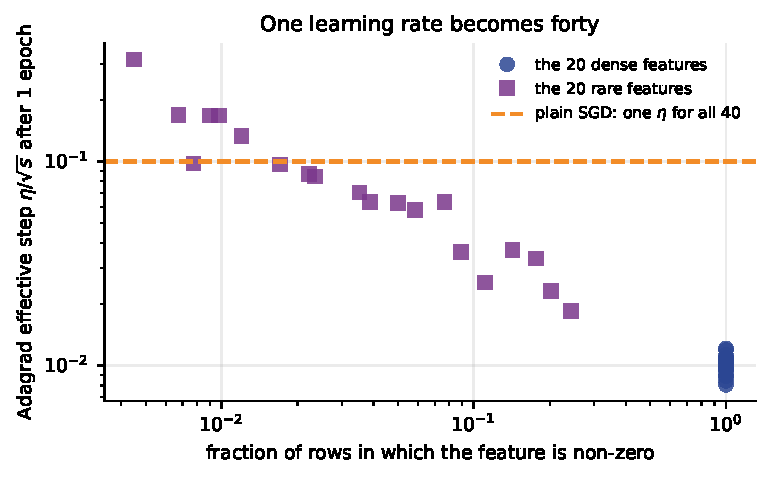
\includegraphics[width=0.58\textwidth]{perparam.pdf}
  \caption{Adagrad's effective step size per coordinate after one epoch of the
  sparse problem, against how often that feature is non-zero, log--log. The
  dashed line is the single $\eta$ that plain SGD would apply to all forty. The
  points fall on a clean trend: the rarer the feature, the larger the step
  Adagrad gives it.}
  \label{fig:perparam}
\end{figure}

Does that translate into recovering the rare weights? It does. At its own best
learning rate, ten epochs of Adagrad lifts the mean of the five rarest weights
from SGD's $0.1562$ to $0.8631$, leaves the dense ones exact at $0.9999$, and
cuts the training MSE from $0.0853$ to $0.0105$. Section~\ref{sec:practice}
puts all five optimisers on the same table.

\begin{keyidea}
If your feature matrix is mostly zeros --- text, one-hot categories,
recommender data, click logs --- try Adagrad before you try anything clever. It
was designed for that case, and on our synthetic version of it, it is worth a
factor of eight in loss and a factor of five in the weights that matter.
\end{keyidea}

\subsection{The flaw: the sum only ever grows}
\label{sec:adagradflaw}

Look at Equation~\eqref{eq:adagrad} again. $s_t = \sum_{k \le t} g_k^2$ is a sum
of squares, so it is non-decreasing, always. It cannot come down.

That would be harmless if the gradients died away, but with mini-batches they
do not. At the optimum the \emph{full} gradient is zero while the individual
mini-batch gradients are not --- that is the noise floor from the previous
lecture. So $s_t$ keeps growing even after training has finished, and the
effective step keeps falling.

\begin{lstlisting}
st["s"] += g*g                        # Adagrad on load_diabetes, eta=0.05
w = w - eta*g/(np.sqrt(st["s"]) + 1e-8)
...
print("update %5d   s = %8.3f   effective step = %.5f"
      % (t, st["s"][2], eta/np.sqrt(st["s"][2])))
\end{lstlisting}
\begin{codeout}
update     1   s =    1.667   effective step = 0.03873
update    10   s =    4.958   effective step = 0.02245
update   100   s =   11.477   effective step = 0.01476
update  1000   s =   58.171   effective step = 0.00656
update  2800   s =  148.007   effective step = 0.00411
after 200 epochs                   MSE 0.4845
\end{codeout}

You asked for $\eta = 0.05$. By update $2800$ this coordinate is being moved
with an effective step of $0.00411$ --- $9.4$ times smaller --- and nothing in
the algorithm will ever let it recover. The rate of decay is easy to predict:
once training has settled each update adds roughly the same $\bar g^2$ to $s$,
so $s_t \approx t\,\bar g^2$ and

\begin{equation}
  \label{eq:adagraddecay}
  \frac{\eta}{\sqrt{s_t}} \;\approx\; \frac{\eta}{\bar g \sqrt{t}}
  \;\propto\; \frac{1}{\sqrt{t}} .
\end{equation}

Adagrad therefore imposes a learning-rate schedule that you did not ask for and
cannot switch off.

\begin{caution}[The $1/\sqrt{t}$ decay is a feature and a fault]
On a convex problem it is a \textbf{feature}: it is precisely the
Robbins--Monro schedule that makes stochastic gradient descent converge rather
than orbit, which is why Adagrad has a convergence proof and RMSprop does not.
Our own run reached MSE $0.4845$ against an optimum of $0.4823$.

On a deep network it is a \textbf{fault}: the loss surface is not convex, the
useful directions change over training, and an optimiser whose step has decayed
to $10^{-4}$ after the first few thousand updates simply stops learning. That
one observation is why RMSprop, Adadelta and Adam all exist.
\end{caution}

\subsection{How bad is the stall? A measurement}

Here is the failure in its purest form: a one-dimensional bowl with its minimum
at $w = 50$, started at $w = 0$, with gradient noise of standard deviation $20$
that never dies away. The inner line is \texttt{s = (s + g*g) if kind ==
"adagrad" else (0.9*s + 0.1*g*g)}; everything else, including $\eta = 0.5$, is
identical between the two runs.
\begin{codeout}
adagrad  t=100   w=  9.01 step=0.00055  t=1000  w= 26.50 step=0.00023
         t=5000  w= 44.80 step=0.00017  t=20000 w= 50.05 step=0.00013
rmsprop  t=100   w= 44.49 step=0.01784  t=1000  w= 50.63 step=0.02488
         t=5000  w= 53.46 step=0.02873  t=20000 w= 48.60 step=0.02334
the minimum is at w = 50
\end{codeout}

Adagrad does arrive --- $50.05$ after twenty thousand updates is an excellent
answer --- but it takes $4874$ updates to reach the point RMSprop reached in
$100$, and by then its step has collapsed to $1.3\times10^{-4}$. If the minimum
were now to move, which is exactly what happens inside a neural network as the
layers below a weight change, Adagrad could no longer follow it. The second row
of that output is the whole of the next section.

Read the RMSprop row again, though, because it is not an unqualified win. Its
$w$ arrives fast and then \emph{wanders}: $50.63$, then $53.46$, then $48.60$.
Its step never shrank, so it never settled. That is the price, and
Section~\ref{sec:rmsprop} charges it explicitly.

% =========================================================================
\section{RMSprop}
\label{sec:rmsprop}

\subsection{One symbol changes}

Adagrad's problem is that $s_t$ is a \emph{sum}. Replace it with an
\emph{average}:

\begin{equation}
  \label{eq:rmsprop}
  s_t = \gamma\, s_{t-1} + (1-\gamma)\, g_t \odot g_t,
  \qquad
  w \;\leftarrow\; w \;-\; \frac{\eta}{\sqrt{s_t} + \varepsilon} \odot g_t ,
\end{equation}

with $\gamma = 0.9$ by default. The second line is unchanged. That is the
entire difference between Adagrad and RMSprop.

You have met this recursion before: it is the same exponentially weighted
average as momentum, in the ``true average'' convention. Unrolling it from
$s_0 = 0$ gives
$s_t = (1-\gamma)\sum_{j=0}^{t-1} \gamma^{\,j} g_{t-j}^2$ with
$(1-\gamma)\sum_{j\ge0}\gamma^{\,j} = 1$, so $s_t$ is a weighted mean of past
squared gradients with total weight $1$, remembering roughly the last
$1/(1-\gamma) = 10$ of them. Because the weights sum to one rather than
growing, $s_t$ stays on the scale of a typical $g^2$ and \emph{can decrease}.
That is the property Adagrad lacked.

RMSprop was proposed by Geoffrey Hinton in lecture 6e of his 2012 Coursera
course and was never published; it is universally cited as ``Hinton,
unpublished'', which is unusual and completely genuine.

\subsection{By hand}

\begin{worked}[Three steps of RMSprop on the same bowl]
Same $f(w) = (w-3)^2$, same $\eta = 0.5$, same start $w_0 = 0$, now with
$\gamma = 0.9$.

\textbf{Step 1.} $g_1 = -6$, so $s_1 = 0.9(0) + 0.1(36) = 3.6$ and
$\sqrt{s_1} = 1.8974$. The step is $0.5(-6)/1.8974 = -1.5811$, giving
$w_1 = 1.5811$.

Compare that with Adagrad's first step of $-0.5$. The two differ by a factor of
$3.1623 = 1/\sqrt{0.1}$, and the reason is visible in the algebra: Adagrad has
$s_1 = g_1^2$ but RMSprop has $s_1 = (1-\gamma)g_1^2$, so

\begin{equation}
  \label{eq:rmsfirst}
  \text{RMSprop's first step} = \frac{\eta}{\sqrt{1-\gamma}}
  \qquad\text{against Adagrad's } \eta .
\end{equation}

At $\gamma = 0.9$ that is $3.16\eta$; at $\gamma = 0.99$ it would be $10\eta$.

\textbf{Step 2.} $g_2 = -2.8377$, so $s_2 = 0.9(3.6) + 0.1(8.053) = 4.0453$,
$\sqrt{s_2} = 2.0113$, step $=-0.7055$, $w_2 = 2.2866$. \textbf{Step 3.}
$g_3 = -1.4268$, so $s_3 = 0.9(4.0453) + 0.1(2.036) = 3.8443$ --- \emph{the
accumulator went down} --- $\sqrt{s_3} = 1.9607$, step $=-0.3639$,
$w_3 = 2.6504$.

\begin{center}
\begin{tabular}{@{}rrrrrr@{}}
\toprule
$t$ & $g_t$ & $s_t = 0.9 s_{t-1} + 0.1 g_t^2$ & $\sqrt{s_t}$ & step & $w_t$\\
\midrule
1 & $-6.0000$ & $3.6000$ & $1.8974$ & $-1.5811$ & $1.5811$\\
2 & $-2.8377$ & $4.0453$ & $2.0113$ & $-0.7055$ & $2.2866$\\
3 & $-1.4268$ & $3.8443$ & $1.9607$ & $-0.3639$ & $2.6504$\\
\bottomrule
\end{tabular}
\end{center}

Adagrad reached $1.0638$ in three steps; RMSprop reached $2.6504$, against a
target of $3$, at an identical learning rate on an identical problem. The whole
difference is row 3: Adagrad's denominator was $8.94$ and climbing, RMSprop's
was $1.96$ and had just fallen.
\end{worked}

\begin{lstlisting}
eta, gamma = 0.5, 0.9
w, s = 0.0, 0.0
for t in (1, 2, 3):
    g = 2.0*(w - 3.0)
    s = gamma*s + (1 - gamma)*g*g            # the only changed line
    w = w - eta*g/(np.sqrt(s) + 1e-8)
    print("t=%d  g=%+8.4f  s=%8.4f  sqrt(s)=%7.4f  step=%+8.4f  w=%.4f"
          % (t, g, s, np.sqrt(s), eta*g/(np.sqrt(s) + 1e-8), w))
\end{lstlisting}
\begin{codeout}
t=1  g= -6.0000  s=  3.6000  sqrt(s)= 1.8974  step= -1.5811  w=1.5811
t=2  g= -2.8377  s=  4.0453  sqrt(s)= 2.0113  step= -0.7055  w=2.2866
t=3  g= -1.4268  s=  3.8443  sqrt(s)= 1.9607  step= -0.3639  w=2.6504
\end{codeout}

Diff the two listings and exactly one line has changed:
\texttt{s = s + g*g} became \texttt{s = gamma*s + (1-gamma)*g*g}.

\subsection{The two denominators, measured}

Two hundred epochs of each on \texttt{load\_diabetes} at $\eta = 0.05$:

\begin{codeout}
adagrad  sqrt(s) after 2800 updates  12.1658   effective step 0.00411
rmsprop  sqrt(s) after 2800 updates   0.1918   effective step 0.26068
\end{codeout}

Over those $2800$ updates Adagrad's denominator rose from $1.29$ to $12.17$
while RMSprop's \emph{fell} from $0.41$ to $0.19$: from the same nominal
$\eta$, Adagrad ended up taking steps $63$ times smaller.

\begin{figure}[tb]
  \centering
  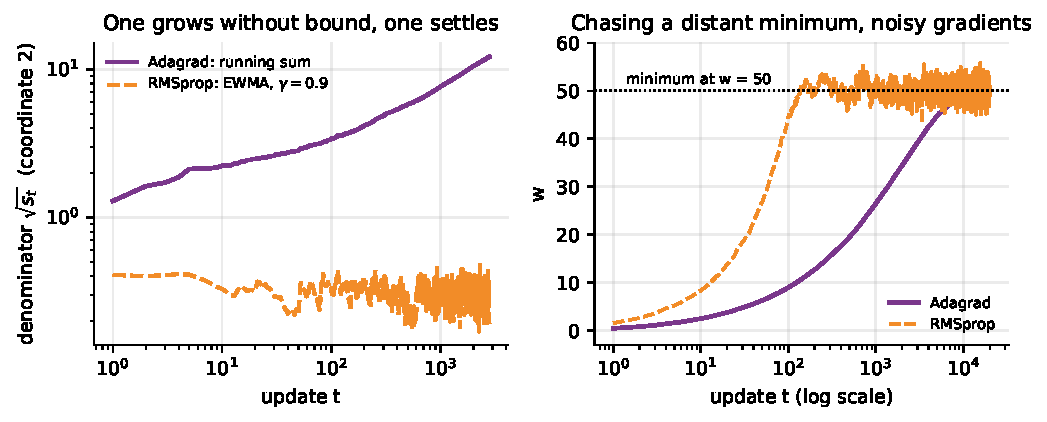
\includegraphics[width=0.76\textwidth]{adagrad_vs_rms.pdf}
  \caption{Left: the denominator $\sqrt{s_t}$ on \texttt{load\_diabetes},
  log--log. Adagrad's grows without bound; RMSprop's settles and then tracks
  the current gradient scale downwards. Right: the cost of that difference ---
  chasing a minimum at $w=50$ through permanent gradient noise, Adagrad is
  still at $9.01$ after $100$ updates where RMSprop is at $44.49$.}
  \label{fig:adagradvsrms}
\end{figure}

\subsection{What RMSprop gives up}

Nothing is free. Adagrad's shrinking step is what guaranteed convergence;
RMSprop's bounded denominator means the step does \emph{not} shrink, so the
iterates never settle --- they orbit the optimum in a noise band whose width is
set by $\eta$, exactly like constant-step SGD. On the 200-epoch run above
Adagrad reached MSE $0.4845$ and RMSprop $0.5310$, against an optimum of
$0.4823$. On a long convex run Adagrad wins.

\begin{keyidea}
Adagrad divides by the square root of a \emph{sum}, so its step decays to zero
and it converges but eventually stalls. RMSprop divides by the square root of
an \emph{average}, so its step stays alive indefinitely and it tracks a moving
target but never settles. Everything else about the two algorithms is
identical.
\end{keyidea}

% =========================================================================
\section{Adadelta}
\label{sec:adadelta}

\subsection{The units are wrong}

Zeiler's 2012 paper starts from an observation that has nothing to do with
convergence rates: it is about \emph{dimensional analysis}. Write $[w]$ for the
units of a parameter and $[J]$ for the units of the loss. A gradient then has
units $[J]/[w]$, and a parameter update must have units $[w]$, because you are
going to add it to $w$.

\begin{center}
\begin{tabular}{@{}lll@{}}
\toprule
\textbf{Method} & \textbf{Update} & \textbf{Units of the update}\\
\midrule
Plain SGD        & $-\eta\, g$              & $[\eta]\,[J]/[w]$\\[3pt]
Adagrad, RMSprop & $-\eta\, g/\sqrt{s}$     & $[\eta]$, because $\sqrt{s}$
                                              cancels $g$ exactly\\[3pt]
Newton           & $-H^{-1} g$              & $[w]$ --- correct, but $H^{-1}$
                                              is unaffordable\\
\bottomrule
\end{tabular}
\end{center}

Only Newton's method has the right units. Plain SGD hides the problem inside
$\eta$, which silently carries units of $[w]^2/[J]$ --- which is why rescaling
your loss forces you to retune it. But look at the middle row: Adagrad and
RMSprop have already done the hard part, because dividing by $\sqrt{s}$ cancels
the gradient's units \emph{completely}. All that is missing is one quantity
carrying the units of $w$, and we have one lying around --- the size of the
updates we have recently been making.

\begin{equation}
  \label{eq:adadeltaidea}
  \Delta w_t \;=\; -\,\frac{\mathrm{RMS}[\Delta w]_{t-1}}{\mathrm{RMS}[g]_t}
  \; g_t .
\end{equation}

There is no $\eta$ anywhere in Equation~\eqref{eq:adadeltaidea}, and that is not
an oversight.

\subsection{The algorithm in full}

Two exponentially weighted averages, one of squared gradients and one of
squared updates:

\begin{align}
  s_t        &= \rho\, s_{t-1} + (1-\rho)\, g_t^2, \label{eq:add1}\\[2pt]
  \Delta w_t &= -\,\frac{\sqrt{d_{t-1} + \varepsilon}}
                        {\sqrt{s_t + \varepsilon}}\; g_t, \label{eq:add2}\\[2pt]
  d_t        &= \rho\, d_{t-1} + (1-\rho)\, \Delta w_t^2, \label{eq:add3}\\[2pt]
  w          &\leftarrow w + \Delta w_t . \label{eq:add4}
\end{align}

Defaults are $\rho = 0.9$ and $\varepsilon = 10^{-6}$. Note two differences
from Adagrad's $\varepsilon$: it sits \emph{inside} both square roots, and it is
ten thousand times larger.

Both of those matter, because $d_0 = 0$. At the very first step
$\mathrm{RMS}[\Delta w]_0 = \sqrt{\varepsilon} = 10^{-3}$, and that number
\emph{is} the initial step-size scale. Adadelta bootstraps itself out of
$\varepsilon$.

\begin{worked}[Adadelta's first step, and why it is tiny]
Same bowl, $f(w) = (w-3)^2$, $w_0 = 0$, $\rho = 0.9$, $\varepsilon = 10^{-6}$.

$g_1 = -6$, so from Equation~\eqref{eq:add1},
$s_1 = 0.1 \times 36 = 3.6$ and $\sqrt{s_1 + \varepsilon} = 1.8974$.
From $d_0 = 0$, $\sqrt{d_0 + \varepsilon} = \sqrt{10^{-6}} = 0.001$. So
\[
  \Delta w_1 = -\,\frac{0.001}{1.8974}\times(-6) = +0.003162,
  \qquad w_1 = 0.003162 .
\]

Adagrad's first step on the same problem was $0.5$; RMSprop's was $1.58$.
Adadelta's is $0.0032$, a hundred and fifty times smaller. Then
$d_1 = 0.1 \times (0.003162)^2 = 10^{-6}$, so
$\sqrt{d_1 + \varepsilon} = 0.001414$ --- the numerator has grown by a factor of
$\sqrt{2}$, and it will keep growing for as long as the steps keep being taken.
\end{worked}

\begin{lstlisting}
rho, epsd = 0.9, 1e-6
w, s, dacc = 0.0, 0.0, 0.0
print("%3s %8s %10s %14s %10s %10s"
      % ("t", "g", "RMS[g]_t", "RMS[dw]_{t-1}", "dw", "w"))
for t in range(1, 201):
    g = 2.0*(w - 3.0)
    s = rho*s + (1 - rho)*g*g
    rms_g  = np.sqrt(s + epsd)            # RMS[g] at step t
    rms_dw = np.sqrt(dacc + epsd)         # RMS[dw] carried in from step t-1
    dw = -rms_dw/rms_g * g
    dacc = rho*dacc + (1 - rho)*dw*dw
    w = w + dw
    if t in (1, 2, 3, 10, 50, 200):
        print("%3d %8.4f %10.4f %14.6f %10.6f %10.6f"
              % (t, g, rms_g, rms_dw, dw, w))
\end{lstlisting}
\begin{codeout}
  t        g   RMS[g]_t  RMS[dw]_{t-1}         dw          w
  1  -6.0000     1.8974       0.001000   0.003162   0.003162
  2  -5.9937     2.6139       0.001414   0.003243   0.006405
  3  -5.9872     3.1199       0.001718   0.003297   0.009702
 10  -5.9397     4.8137       0.002825   0.003485   0.033635
 50  -5.6428     5.6952       0.003932   0.003896   0.182487
200  -4.3511     4.4339       0.004662   0.004575   0.829020
\end{codeout}

After two hundred steps $w$ has reached only $0.83$ out of $3$. On this small,
well-conditioned, noiseless problem Adadelta is dramatically slower than
everything else. The slow start is real and it is inherent: the numerator has
to grow from $\sqrt{\varepsilon}$ to whatever the right scale is, and it can
only do that by taking steps.

\begin{caution}[$\varepsilon$ is Adadelta's hidden learning rate]
Because the first step is $\sqrt{\varepsilon}\,|g_1|/\mathrm{RMS}[g]_1$, the
size of the first step is proportional to $\sqrt{\varepsilon}$. Set
$\varepsilon = 10^{-12}$ instead of $10^{-6}$ and the first step is a thousand
times smaller --- practice question~7 works this out. So Adadelta does not
really have zero hyperparameters; it has one, and it is disguised as a
numerical-stability constant. It is nevertheless a far less sensitive
hyperparameter than $\eta$, because the algorithm corrects for a bad initial
guess automatically.
\end{caution}

\subsection{The step size it works out for itself}

The ratio $r_t = \mathrm{RMS}[\Delta w]_{t-1}/\mathrm{RMS}[g]_t$ in
Equation~\eqref{eq:adadeltaidea} multiplies the gradient, exactly as $\eta$ does
in plain SGD. So it is directly comparable with a learning rate --- and we can
ask what value Adadelta arrives at, and whether it is the value a human would
have chosen.

\begin{lstlisting}
r = np.sqrt(dacc + epsd)/np.sqrt(s + epsd)   # record this, on load_diabetes
dw = -r*g                                    # B=32, 200 epochs
\end{lstlisting}
\begin{codeout}
Adadelta's own step size  r_t = RMS[dw]_{t-1} / RMS[g]_t  (coordinate 2)
   update     1    r = 0.002449
   update    10    r = 0.002558
   update   100    r = 0.005168
   update  1000    r = 0.009843
   update  2800    r = 0.012292
   median r over the last epoch, all 10 coords    0.012427
   the eta a human found by search for plain SGD  0.005000
   final MSE 0.4840   (optimum 0.4823)
\end{codeout}

Read the last two lines together. A human tuned plain SGD by grid search and
settled on $\eta = 0.005$; Adadelta, told nothing, worked its way from $0.0024$
up to $0.0124$ and landed within a factor of two and a half of that --- on the
correct side, since by the end of training a larger step is affordable.

\subsection{Dimensional consistency, tested}

The units argument makes a falsifiable prediction. Multiply the loss by a
constant $c$: every gradient is multiplied by $c$, the optimum stays exactly
where it was, and the problem is in every sense unchanged. A dimensionally
consistent optimiser should behave identically; a learning rate should have to
be re-tuned by $1/c$.

\begin{lstlisting}
g = c*grad(X[idx], y[idx], w)     # the only change: the loss is c times bigger
\end{lstlisting}
\begin{codeout}
multiply the loss by c; nothing else changes.  30 epochs, B=32
c           SGD eta=0.005       Adadelta
0.01               0.8941         0.4860
1                  0.4860         0.4859
100              diverged         0.4859
least-squares optimum                     0.4823
\end{codeout}

SGD at a fixed $\eta$ is useless at $c = 0.01$ --- effectively a learning rate
a hundred times too small --- and blows up at $c = 100$. Adadelta returns
$0.4860$, $0.4859$, $0.4859$; over a nine-point sweep of $c$ spanning four
decades its answer varies by a factor of $1.0002$.

\begin{figure}[tb]
  \centering
  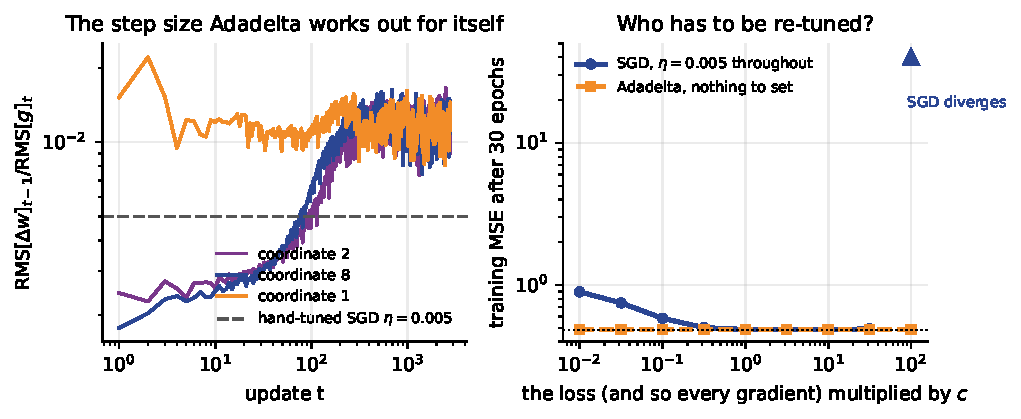
\includegraphics[width=0.76\textwidth]{adadelta.pdf}
  \caption{Left: the step size $r_t$ that Adadelta computes for itself on
  \texttt{load\_diabetes}, three coordinates, against the hand-tuned SGD
  learning rate of $0.005$ (dashed). It starts far below it, climbs, and
  settles slightly above. Right: multiply the loss by $c$ and see who has to be
  re-tuned. Adadelta is a flat line across four decades; SGD is wrong at both
  ends and diverges at $c = 100$.}
  \label{fig:adadelta}
\end{figure}

On \texttt{load\_diabetes} with $B = 32$ and no learning rate supplied,
Adadelta reaches MSE $0.5665$ after five epochs and $0.4859$ after thirty,
against an optimum of $0.4823$. The second number is as good as hand-tuned SGD
($0.4860$) with nothing tuned at all; the first is the worst of the six
optimisers compared in Section~\ref{sec:practice}.

\begin{keyidea}
Adadelta is the answer to a question nobody else asked: what would an optimiser
look like if its update had the same units as the parameter? The answer needs
no learning rate, is invariant to rescaling the loss, and pays for both with the
slowest start of any method here.
\end{keyidea}

One implementation note: PyTorch's \texttt{Adadelta} still takes an \texttt{lr},
defaulting to $1.0$. It is a pure gain on $\Delta w$ in
Equation~\eqref{eq:add2}, not a step size, and $1.0$ means ``as published''.
Leave it there unless you have a measured reason not to.

% =========================================================================
\section{Adam}
\label{sec:adam}

\subsection{Momentum plus RMSprop}

Adam --- \textbf{Ada}ptive \textbf{M}oment estimation --- puts the two ideas
together. Momentum averages the gradient to fix the direction; RMSprop averages
the squared gradient to fix the scale. Adam keeps both averages and divides one
by the square root of the other.

\begin{align}
  m_t &= \beta_1 m_{t-1} + (1-\beta_1)\, g_t
    &&\text{first moment: direction, from momentum} \label{eq:adam1}\\
  v_t &= \beta_2 v_{t-1} + (1-\beta_2)\, g_t^2
    &&\text{second moment: scale, from RMSprop} \label{eq:adam2}\\
  \hat m_t &= \frac{m_t}{1-\beta_1^{\,t}}, \qquad
  \hat v_t = \frac{v_t}{1-\beta_2^{\,t}}
    &&\text{bias correction} \label{eq:adam3}\\
  w &\leftarrow w - \frac{\eta\, \hat m_t}{\sqrt{\hat v_t} + \varepsilon}
    &&\text{the step} \label{eq:adam4}
\end{align}

The defaults from Kingma and Ba's 2015 paper are $\beta_1 = 0.9$,
$\beta_2 = 0.999$, $\varepsilon = 10^{-8}$ and $\eta = 0.001$, and they are what
every framework ships.

Notice that Equation~\eqref{eq:adam1} uses the \emph{other} momentum convention:
$m$ is a true running average with the $(1-\beta_1)$ factor, not
$v \leftarrow \beta v + g$. That choice is what makes the bias-correction line
necessary, and it is the subject of the next subsection.

\subsection{Why the first steps are biased}

Both averages start at zero. Unrolling one step gives
$m_1 = (1-\beta_1) g_1 = 0.1\,g_1$ and
$v_1 = (1-\beta_2) g_1^2 = 0.001\,g_1^2$: both are pulled towards their initial
value of zero, $m_1$ to one tenth of $g_1$ and $v_1$ to one thousandth of
$g_1^2$. The general statement is easy --- if the gradient were exactly
constant at $g$ then unrolling Equation~\eqref{eq:adam1} gives
$m_t = (1-\beta_1)\sum_{j=0}^{t-1}\beta_1^{\,j} g = (1-\beta_1^{\,t})\, g$, so
dividing by $1-\beta_1^{\,t}$ recovers $g$ exactly. That is
Equation~\eqref{eq:adam3}, and the same argument gives the $\beta_2$ half.

Now the crucial point, and the one students most often miss.

\begin{keyidea}[The problem is the mismatch, not the shrinkage]
If both moments were shrunk by the \emph{same} factor, the ratio
$m/\sqrt{v}$ would be unaffected and no correction would be needed. But $m$ is
shrunk by $1-\beta_1 = 0.1$ while $\sqrt{v}$ is shrunk by
$\sqrt{1-\beta_2} = \sqrt{0.001} = 0.0316$. They do not cancel. The ratio comes
out
\[
  \frac{0.1}{0.0316} = \frac{1-\beta_1}{\sqrt{1-\beta_2}} = 3.1623
\]
times too \textbf{large}. Bias correction exists because $\beta_1$ and
$\beta_2$ are different numbers.
\end{keyidea}

\subsection{Adam by hand}

\begin{worked}[Adam, step 1, on $f(w)=(w-3)^2$]
Take $\eta = 0.1$, $\beta_1 = 0.9$, $\beta_2 = 0.999$, $w_0 = 0$,
$m_0 = v_0 = 0$.

\begin{center}
\begin{tabular}{@{}ll@{}}
\toprule
gradient       & $g_1 = 2(0-3) = -6$\\[3pt]
first moment   & $m_1 = 0.9(0) + 0.1(-6) = -0.6$\\[3pt]
second moment  & $v_1 = 0.999(0) + 0.001(36) = 0.036$\\[3pt]
correct $m$    & $\hat m_1 = -0.6/(1-0.9) = -0.6/0.1 = -6$\\[3pt]
correct $v$    & $\hat v_1 = 0.036/(1-0.999) = 0.036/0.001 = 36$\\[3pt]
denominator    & $\sqrt{\hat v_1} = 6$\\[3pt]
step           & $\Delta w = -0.1 \times (-6)/6 = +0.1$\\[3pt]
\textbf{new parameter} & $\mathbf{w_1 = 0.1}$\\
\bottomrule
\end{tabular}
\end{center}

Look at the two corrected quantities: $\hat m_1 = g_1$ and
$\hat v_1 = g_1^2$, \emph{exactly}. That is not a coincidence of the numbers; it
is what the correction is for. So the corrected first step is always
\[
  -\eta\,\frac{g_1}{|g_1|} = \pm\eta .
\]

\textbf{Adam's first step has size exactly $\eta$, in the downhill direction,
whatever the magnitude of the gradient.} This is the single most useful fact
about Adam in practice: it tells you what $\eta$ means. Set $\eta = 0.001$ and
you are saying ``move each parameter by about $0.001$ per step''.
\end{worked}

\begin{worked}[Adam, steps 2 and 3]
Carry $w_1 = 0.1$, $m_1 = -0.6$, $v_1 = 0.036$ forward.

$g_2 = 2(0.1-3) = -5.8$, so $m_2 = 0.9(-0.6) + 0.1(-5.8) = -1.12$ and
$v_2 = 0.999(0.036) + 0.001(33.64) = 0.069604$. The correction factors at
$t=2$ are $1-\beta_1^2 = 0.19$ and $1-\beta_2^2 = 0.001999$, so
\[
  \hat m_2 = \frac{-1.12}{0.19} = -5.8947,
  \qquad
  \hat v_2 = \frac{0.069604}{0.001999} = 34.819,
  \qquad \sqrt{\hat v_2} = 5.9008 ,
\]
and the step is $-0.1 \times (-5.8947)/5.9008 = +0.099897$, giving
$w_2 = 0.199897$. Step 3 works the same way and gives $w_3 = 0.299618$.

\begin{center}
\begin{tabular}{@{}rrrrrrr@{}}
\toprule
$t$ & $g_t$ & $m_t$ & $v_t$ & $\hat m_t$ & $\sqrt{\hat v_t}$ & $w_t$\\
\midrule
1 & $-6.0000$ & $-0.60000$ & $0.036000$ & $-6.0000$ & $6.0000$ & $0.100000$\\
2 & $-5.8000$ & $-1.12000$ & $0.069604$ & $-5.8947$ & $5.9008$ & $0.199897$\\
3 & $-5.6002$ & $-1.56802$ & $0.100897$ & $-5.7861$ & $5.8022$ & $0.299618$\\
\bottomrule
\end{tabular}
\end{center}

The three steps are $0.1000$, $0.0999$, $0.0997$. Adam is moving at almost
exactly the speed you asked for, and it will keep doing so until the gradient
changes sign or the sign pattern becomes inconsistent. The ratio
$\hat m/\sqrt{\hat v}$ stays near $\pm 1$ because both moments are tracking the
\emph{same} sequence of gradients.
\end{worked}

\begin{lstlisting}
eta, b1, b2, eps = 0.1, 0.9, 0.999, 1e-8
w, m, v = 0.0, 0.0, 0.0
print("%3s %9s %10s %10s %10s %11s %10s"
      % ("t", "g", "m", "v", "mhat", "sqrt(vhat)", "w"))
for t in (1, 2, 3):
    g = 2.0*(w - 3.0)
    m = b1*m + (1 - b1)*g
    v = b2*v + (1 - b2)*g*g
    mh, vh = m/(1 - b1**t), v/(1 - b2**t)          # bias correction
    w = w - eta*mh/(np.sqrt(vh) + eps)
    print("%3d %9.4f %10.5f %10.6f %10.4f %11.4f %10.6f"
          % (t, g, m, v, mh, np.sqrt(vh), w))
\end{lstlisting}
\begin{codeout}
  t         g          m          v       mhat  sqrt(vhat)          w
  1   -6.0000   -0.60000   0.036000    -6.0000      6.0000   0.100000
  2   -5.8000   -1.12000   0.069604    -5.8947      5.9008   0.199897
  3   -5.6002   -1.56802   0.100897    -5.7861      5.8022   0.299618
\end{codeout}

Six lines of arithmetic. Adam is Adagrad's per-coordinate idea, RMSprop's fix
for it, momentum's direction, and two divisions.

\subsection{How wrong is the uncorrected version?}

\begin{lstlisting}
b1, b2, g1 = 0.9, 0.999, -6.0
m1, v1 = (1 - b1)*g1, (1 - b2)*g1*g1
print("uncorrected  m1 / sqrt(v1)   = %+.4f" % (m1/np.sqrt(v1)))
print("corrected    mhat1/sqrt(vhat1) = %+.4f"
      % ((m1/(1 - b1))/np.sqrt(v1/(1 - b2))))
tt = np.arange(1, 20001)
ratio = (1/(1 - b1**tt))/np.sqrt(1/(1 - b2**tt))   # corrected / uncorrected
\end{lstlisting}
\begin{codeout}
first gradient                g1        = -6.0000
uncorrected  m1 / sqrt(v1)              = -3.1623
corrected    mhat1 / sqrt(vhat1)        = -1.0000
ratio  (1-b1)/sqrt(1-b2)                = 3.1623
worst overshoot at t=12, factor 6.57 too big
within 1% of the corrected step only from t=3916
\end{codeout}

Three facts there, all worth remembering. At $t=1$ the uncorrected step is
$3.16$ times too big. It then gets \emph{worse}, peaking at $6.57$ times too
big at $t=12$, because $1-\beta_1^t$ recovers quickly (within $1\%$ of $1$ by
step $44$) while $1-\beta_2^t$ recovers slowly (step $4613$), so for a few
hundred steps the numerator is essentially correct while the denominator is
still far too small. And the two do not agree to within one per cent until step
$3916$: on a short run --- and many fine-tuning runs are a few thousand steps
--- \emph{the whole run} is inside the biased region.

\subsection{The two trajectories, run side by side}

Ratios are abstract. Here are the two runs themselves --- identical code,
identical $\eta$, the only difference being whether
Equation~\eqref{eq:adam3} is applied.

\begin{lstlisting}
mh, vh = (m/(1 - b1**t), v/(1 - b2**t)) if bias_correct else (m, v)
\end{lstlisting}
\begin{codeout}
f(w)=(w-3)^2, w0=0, eta=0.1, 80 steps
               t=1       t=2       t=3       t=12
w, corrected   0.1000    0.1999    0.2996    1.1753
w, no bc       0.3162    0.7393    1.2263    4.4123
step size, corrected: never exceeds 0.1000  (you asked for 0.1)
step size, no bc:     peaks at      0.5340  = 5.3 times too big
furthest past the minimum, corrected  3.1773 at t=53
furthest past the minimum, no bc      4.4123 at t=12
\end{codeout}

The corrected run does what it was told: no step ever exceeds $0.1000$, and it
approaches the minimum from below, overshooting only to $3.1773$. The
uncorrected run takes steps of up to $0.5340$ when you asked for $0.1$, and by
step $12$ --- the exact step the theory predicted as the worst --- it is at
$4.4123$, a long way past a minimum at $3$. On this convex bowl it oscillates
back and recovers; on a loss surface with several basins it would have left the
one you started in.

\begin{figure}[tb]
  \centering
  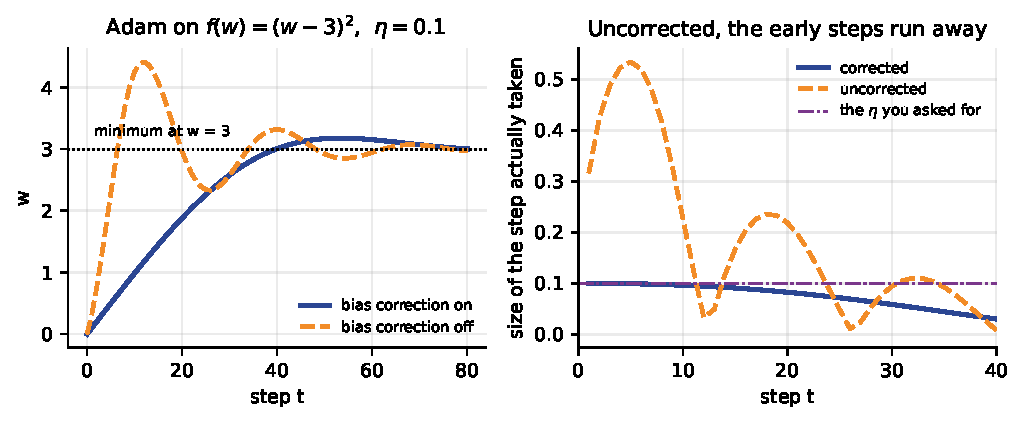
\includegraphics[width=0.76\textwidth]{adam_traj.pdf}
  \caption{Adam on $f(w)=(w-3)^2$ with $\eta=0.1$, with and without the two
  bias-correction lines. Left: the trajectories. Right: the size of the step
  actually taken at each iteration, against the $\eta$ that was requested. The
  uncorrected run's step peaks at $0.534$ around $t=5$ and is still oscillating
  at $t=40$.}
  \label{fig:adamtraj}
\end{figure}

\subsection{Does it matter on a real fit?}

\begin{lstlisting}
print("Adam, eta=0.02, B=32          epoch 1   epoch 5   epoch 30")
for bc in (True, False):
    hh, _, _ = run(X, y, "adam", 0.02, epochs=30, bias_correct=bc)
    print("bias correction %-3s            %7.4f   %7.4f    %7.4f"
          % ("on" if bc else "off", hh[1], hh[5], hh[30]))
\end{lstlisting}
\begin{codeout}
Adam, eta=0.02, B=32          epoch 1   epoch 5   epoch 30
bias correction on              0.5369    0.4888     0.4929
bias correction off             0.5758    0.4885     0.4960
\end{codeout}

Honest answer: on a convex ten-parameter problem, barely. The first epoch is
measurably worse without correction ($0.5758$ against $0.5369$) and by epoch
five the two are indistinguishable.

It is in the algorithm anyway for three reasons. On a large non-convex model
the first few hundred oversized steps can move you into a region you never
recover from --- our bowl was forgiving, a transformer is not. \textbf{An
$\eta$ tuned with correction is not an $\eta$ tuned without it}, so if your
framework corrects and your reimplementation does not, every learning rate you
have ever tuned is wrong by up to $6.6\times$ during the period that matters
most. And it costs two divisions.

\begin{keyidea}[The modern descendant]
\textbf{Warmup} --- linearly ramping $\eta$ from zero over the first few
thousand steps --- is doing the same job as bias correction, more crudely and
more forcefully, and for the same reason: the second-moment estimate is
unreliable when it has seen only a handful of gradients. If you ever wondered
why large-model training recipes all begin with a warmup, this is why.
\end{keyidea}

% =========================================================================
\section{Numerical practice}
\label{sec:practice}

We now have five optimisers plus plain SGD. This section is the part that
actually changes what you do on Monday.

\subsection{All six on the same problem}

\begin{lstlisting}
for kind, e in (("sgd", 0.005), ("momentum", 0.005), ("adagrad", 0.05),
                ("rmsprop", 0.005), ("adadelta", 1.0), ("adam", 0.02)):
    hh, _, _ = run(X, y, kind, e, epochs=30)
\end{lstlisting}
\begin{codeout}
optimiser     eta    epoch 1  epoch 5 epoch 30
sgd         0.005     0.7393   0.5358   0.4860
momentum    0.005     0.5711   0.4870   0.4846
adagrad     0.050     0.5349   0.4884   0.4859
rmsprop     0.005     0.6613   0.4948   0.4853
adadelta    1.000     0.8157   0.5665   0.4859
adam        0.020     0.5369   0.4888   0.4929
optimum                                 0.4823
\end{codeout}

Read the last column before the first. All six land between $0.4846$ and
$0.4929$, against an optimum of $0.4823$: the spread across the entire family
is under two per cent, the winner is plain momentum, and Adam --- the universal
default --- is \emph{last}.

\begin{figure}[tb]
  \centering
  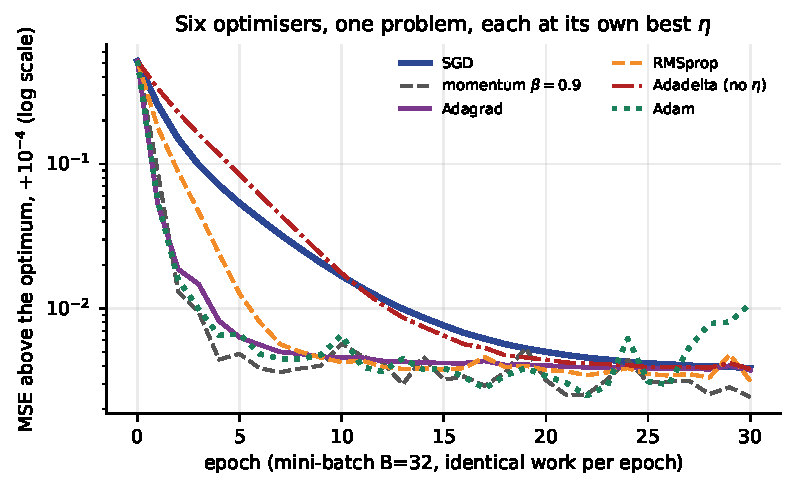
\includegraphics[width=0.62\textwidth]{optimcompare.pdf}
  \caption{The same six runs, plotted as distance above the optimum on a log
  scale. The adaptive methods win the first two epochs decisively and then
  flatten into a noise band; momentum descends more slowly at first and keeps
  going. Reading only the first epoch would give you the opposite conclusion
  from reading the last.}
  \label{fig:optimcompare}
\end{figure}

\begin{caution}[The most common wrong conclusion in this whole lecture]
``Adam is better'' and ``Adam is worse'' are both unsupportable from that
table. On a well-conditioned convex problem with a tuned learning rate the
choice of optimiser is worth about one per cent. If you are choosing an
optimiser to gain one per cent, go and look at your features instead.
\end{caution}

\subsection{Where the choice does matter}

Now run the same comparison on the \emph{sparse} problem.

\begin{codeout}
optimiser     eta        MSE     dense  5 rarest
sgd         0.010     0.0853    1.0004   0.1562
momentum    0.001     0.0853    0.9998   0.1557
adagrad     0.100     0.0105    0.9999   0.8631
rmsprop     0.005     0.0106    1.0003   0.9846
adam        0.050     0.0125    0.9990   1.0051
\end{codeout}

Here the choice of optimiser is worth a factor of eight in loss and a factor of
six in the weights you care about. Note momentum: indistinguishable from plain
SGD, because averaging the \emph{direction} does nothing for a coordinate whose
gradient is zero nine times in ten. Every \emph{per-coordinate} method fixes
it; the one non-per-coordinate method does not.

\begin{figure}[tb]
  \centering
  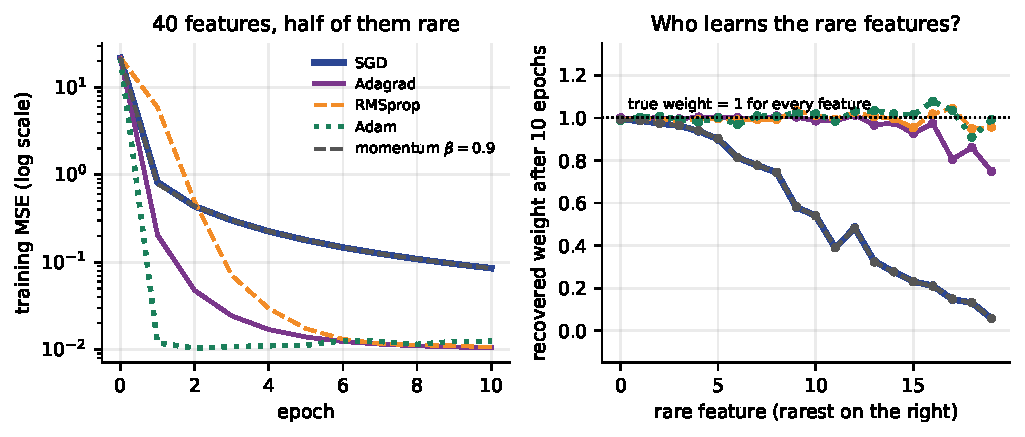
\includegraphics[width=0.76\textwidth]{sparse.pdf}
  \caption{Left: training MSE per epoch on the sparse problem. Right: the
  weight each method recovered for each of the twenty rare features, rarest on
  the right, against a true value of $1$. SGD and momentum fall away as the
  features get rarer; Adam and RMSprop hold up across the whole range.}
  \label{fig:sparse}
\end{figure}

\begin{keyidea}
Adaptive optimisers are not a general-purpose improvement. They are a specific
remedy for \emph{heterogeneity between parameters} --- some rare, some common,
some steep, some shallow. On a homogeneous problem they buy you almost nothing;
on a heterogeneous one they are the difference between learning a feature and
not learning it.
\end{keyidea}

\subsection{The real benefit: a wider target to aim at}

There is a second benefit, and it is the one that explains why practitioners
reach for Adam by reflex. It is not about the final number; it is about how
hard it is to find a working learning rate.

\begin{lstlisting}
etas = np.geomspace(1e-4, 3.0, 25)
for kind in ("sgd", "momentum", "adagrad", "rmsprop", "adam"):
    good = [e for e in etas
            if run(X, y, kind, float(e), epochs=10)[0][-1] < 1.05*mse(X, y, w_star)]
    print("%-10s %2d/25 grid points work:  %.4f to %.4f  (%.2f decades)"
          % (kind, len(good), min(good), max(good),
             np.log10(max(good)/min(good))))
\end{lstlisting}
\begin{codeout}
sgd         8/25 grid points work:  0.0048 to 0.0965  (1.31 decades)
momentum   10/25 grid points work:  0.0006 to 0.0266  (1.68 decades)
adagrad    13/25 grid points work:  0.0173 to 3.0000  (2.24 decades)
rmsprop     9/25 grid points work:  0.0020 to 0.0628  (1.49 decades)
adam        9/25 grid points work:  0.0031 to 0.0965  (1.49 decades)
\end{codeout}

Adagrad works over $2.24$ decades of learning rate against plain SGD's $1.31$,
and $3.0$ is where our grid stopped rather than where Adagrad failed. Its own
$1/\sqrt{t}$ decay rescues a learning rate that would destroy any other method
within a few updates.

\begin{figure}[tb]
  \centering
  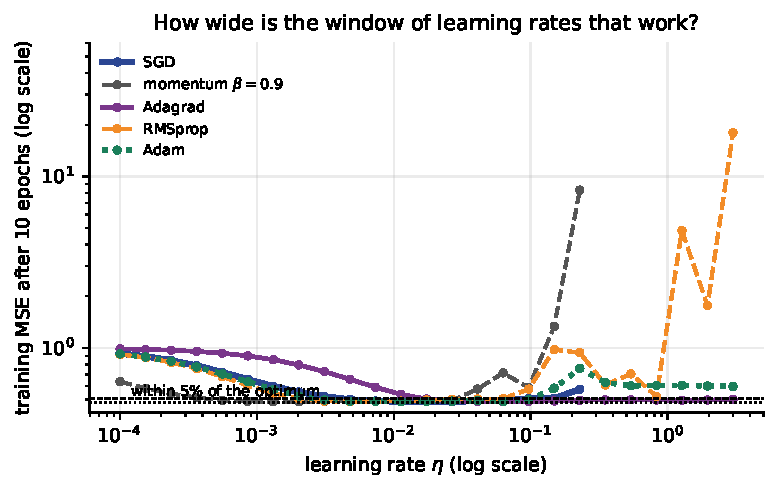
\includegraphics[width=0.62\textwidth]{lrsensitivity.pdf}
  \caption{Training MSE after ten epochs against learning rate, log--log. Every
  curve is a bathtub with a soft left wall and a hard right one: too small is
  merely slow, too large is fatal. The width of the flat bottom is what an
  adaptive optimiser buys you.}
  \label{fig:lrsensitivity}
\end{figure}

\begin{keyidea}[What adaptive optimisers actually buy]
Not a better final answer --- one per cent, on our data --- but a \textbf{wider
window of learning rates that work}. On a problem you have never seen, where
each trial costs an hour, that is worth far more than one per cent.
\end{keyidea}

\subsection{The ravine, revisited}

The previous lecture's ravine, $f(w) = 0.01w_1^2 + 2w_2^2$ with $\kappa = 200$,
is deterministic, dense and purely a curvature problem. It is the case adaptive
methods are \emph{not} designed for, and the measurement says so.

\begin{codeout}
optimiser      eta   iters to ||w||<1e-3  ||w|| after 1200
gd           0.475                   954          9.99e-04
momentum     0.475                   135          7.88e-04
adagrad      0.500                   805          9.97e-04
rmsprop      0.050                 never          3.54e-02
adam         0.100                   262          9.89e-04
\end{codeout}

Momentum wins outright at $135$ iterations, with Adam second at $262$ and
Adagrad barely ahead of plain gradient descent. Two things explain this.

A ravine is defined by \emph{curvature} and adaptive methods measure
\emph{gradients}, so they are reading the wrong quantity: a coordinate can have
a small gradient because the surface is flat there or because it happens to be
near its own optimum, and $\sqrt{s}$ cannot tell those apart. Momentum's
acceleration is by contrast a genuine $\kappa \to \sqrt{\kappa}$ improvement in
the rate. RMSprop never reaches the tolerance at all: its denominator is
bounded and its $\eta$ constant, so the step does not go to zero and it settles
into a limit cycle at $3.5\times10^{-2}$ --- not slow convergence, but not
converging.

\begin{figure}[tb]
  \centering
  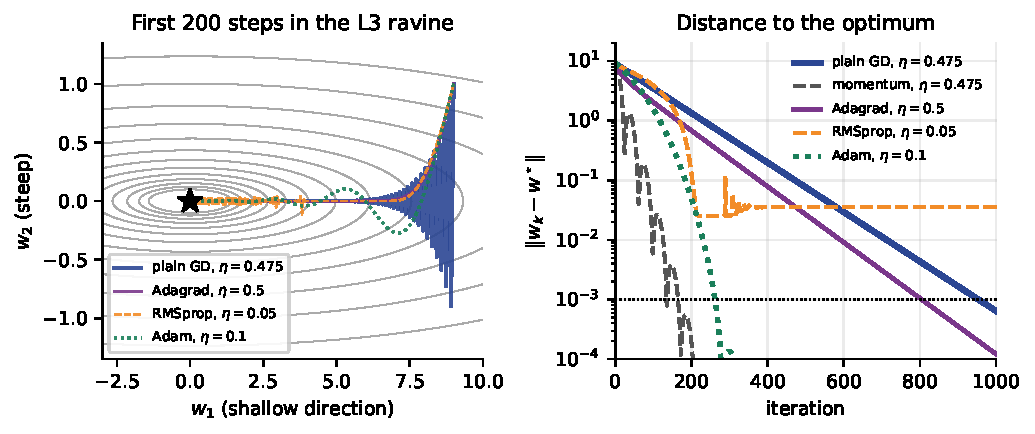
\includegraphics[width=0.76\textwidth]{ravine_adaptive.pdf}
  \caption{Left: the first $200$ steps in the ravine. Right: distance to the
  optimum on a log scale, where a straight line is geometric convergence; the
  flat orange line is RMSprop's limit cycle.}
  \label{fig:ravineadaptive}
\end{figure}

\subsection{Two numerical details that will cost you a run}

\subsubsection*{Where $\varepsilon$ goes, and how big it is}

Ten epochs of RMSprop at $\eta = 0.005$, sweeping \texttt{eps}:

\begin{codeout}
RMSprop, epsilon =   1e-08   MSE after 10 epochs 0.4864
RMSprop, epsilon =   1e-04   MSE after 10 epochs 0.4864
RMSprop, epsilon =   1e-02   MSE after 10 epochs 0.4864
RMSprop, epsilon =   1e-01   MSE after 10 epochs 0.4870
RMSprop, epsilon =   1e+00   MSE after 10 epochs 0.5185
\end{codeout}

Anything at or below $10^{-2}$ is identical to four decimal places (the
$10^{-6}$ row, omitted above, reads $0.4864$ too). At $\varepsilon = 1$ it
dominates $\sqrt{s}$, the denominator becomes a constant, and RMSprop
degenerates into plain SGD with a smaller learning rate. There is also the
question of \emph{where} it goes: our rule, D2L's and PyTorch's \texttt{Adam}
put it outside the root, $\sqrt{s} + \varepsilon$, Keras and PyTorch's
\texttt{RMSprop} inside, $\sqrt{s + \varepsilon}$. At $\varepsilon = 10^{-2}$
the two give $0.486409$ and $0.486443$.

\begin{caution}[Adam's $\varepsilon$ is a hyperparameter in one specific case]
If whole coordinates receive zero gradient for long stretches --- sparse
embeddings, mixture-of-experts routing --- then $\sqrt{\hat v}$ really does
approach zero and $\varepsilon$ really does set the maximum step. Practitioners
there raise it to $10^{-6}$ or $10^{-4}$. Everywhere else, leave it alone.
\end{caution}

\subsubsection*{Adaptive does not mean schedule-free}

Adam at $\eta = 0.02$, with and without an $\eta_t = \eta_0/(1+ct)$ decay at
$c = 0.004$:

\begin{codeout}
Adam, decay off  epoch  5   MSE 0.4888    epoch 30   MSE 0.4929
Adam, decay on   epoch  5   MSE 0.4877    epoch 30   MSE 0.4850
least-squares optimum                                MSE 0.4823
\end{codeout}

Adam got \emph{worse} between epoch 5 and epoch 30, from $0.4888$ to $0.4929$.
It is not diverging; it has reached its noise floor and is orbiting, and the
orbit is wider than where it happened to be at epoch 5. The decay fixes it:
$0.4850$ at epoch 30.

\begin{caution}[The single most common mistake with Adam]
Believing that ``adaptive'' means it needs no learning-rate schedule. Adam
adapts the \emph{relative} step size between coordinates; the overall
scale is still $\eta$, and $\eta$ still has to come down at the end or you sit
on the noise floor. Cosine, step and linear decay-to-zero are all used, and
which you pick matters far less than doing it at all.
\end{caution}

\subsection{A recipe}

\begin{enumerate}[leftmargin=*]
  \item \textbf{Standardise the features.} Nothing here rescues an
    unstandardised feature matrix; the previous lecture measured a condition
    number going from $470$ to $1.2\times10^8$ from one unit change.
  \item \textbf{Start with Adam, $\eta = 10^{-3}$, $B = 32$.} Widest practical
    window of learning rates, and $\eta$ means the size of an early step.
  \item \textbf{Sweep $\eta$ over powers of ten} for a few epochs each, take
    the largest that does not misbehave, back off by three.
    Figure~\ref{fig:lrsensitivity} is the shape you are looking for.
  \item \textbf{If the features are sparse}, try Adagrad, and expect a large
    difference rather than a marginal one.
  \item \textbf{Decay $\eta$ towards the end.} Always. Even with Adam.
  \item \textbf{If the final number matters}, tune SGD with momentum as a
    competitor: on our data it won, $0.4846$ against Adam's $0.4929$.
\end{enumerate}

\subsection{What the libraries give you}

\begin{sloppypar}
\texttt{torch.optim} contains \texttt{Adagrad}, \texttt{RMSprop},
\texttt{Adadelta} and \texttt{Adam} with exactly these update rules, and their
arguments are the notation used here: \texttt{lr} is $\eta$, \texttt{betas} is
$(\beta_1,\beta_2)$, \texttt{alpha} is RMSprop's $\gamma$, \texttt{rho} is
Adadelta's $\rho$, \texttt{eps} is $\varepsilon$. Read the documentation's
algorithm block before trusting a formula found elsewhere; conventions
genuinely differ between libraries. scikit-learn exposes less:
\texttt{SGDRegressor} has no adaptive option and \texttt{MLPRegressor} takes
\texttt{solver="adam"} with \texttt{learning\_rate\_init}, \texttt{beta\_1},
\texttt{beta\_2} and \texttt{epsilon}. For Adagrad or Adadelta on a linear
model you write the loop: it is the six branches of Section~\ref{sec:why}.
\end{sloppypar}

\begin{tryit}
Re-run the sparse problem of Section~\ref{sec:sparse} with the densities
changed to \texttt{np.geomspace(0.25, 0.05, 20)}, so the rarest feature fires
in $200$ rows rather than $18$. Adagrad's advantage on the five rarest weights
should almost vanish: it is proportional to feature heterogeneity.
\end{tryit}

\newpage
% =========================================================================
\section{Summary}

\begin{enumerate}[leftmargin=*]
  \item A single learning rate fails for two independent reasons:
    \textbf{curvature} (coordinates whose second derivatives differ by $\kappa$
    want steps differing by $\kappa$; in our ravine, $50$ against $0.25$) and
    \textbf{frequency} (a feature firing in $18$ rows out of $4000$ needs a much
    bigger step when it does fire).
  \item Every optimiser in this lecture is
    $w_i \leftarrow w_i - (\eta/\sqrt{s_i})\,g_i$. They differ only in what
    $s_i$ accumulates.
  \item \textbf{Adagrad}: $s_t = s_{t-1} + g_t^2$. It turned one $\eta$ into
    forty, with a spread of $39\times$, and lifted the five rarest weights from
    $0.156$ to $0.863$ while leaving the dense ones exact. Its first step has
    size exactly $\eta$, whatever the gradient. But its accumulator never
    decreases, so the effective step decays like $1/\sqrt{t}$ forever ---
    $9.4\times$ smaller after $2800$ updates and still falling --- and chasing
    a moving target it needed $4874$ updates to reach what RMSprop reached in
    $100$.
  \item \textbf{RMSprop}: replace the sum by $\gamma s + (1-\gamma)g^2$. One
    line. Same bowl, same $\eta$: Adagrad reached $1.064$ in three steps,
    RMSprop $2.650$. RMSprop's first step is $\eta/\sqrt{1-\gamma} = 3.16\eta$,
    not $\eta$.
  \item What RMSprop gives up is convergence: its step never shrinks, so on the
    200-epoch convex run Adagrad reached $0.4845$ and RMSprop $0.5310$.
  \item \textbf{Adadelta}: $\eta g/\sqrt{s}$ has the wrong units; supply
    $\mathrm{RMS}[\Delta w]_{t-1}$ as the numerator and the learning rate
    disappears. It found its own step size of $0.0124$ where a human found
    $0.005$, and multiplying the loss by $100$ changed its answer by $0.02\%$
    while SGD diverged.
    It pays with the slowest start: $0.5665$ at five epochs, worst of the six,
    though $0.4859$ by thirty.
  \item \textbf{Adam} is momentum $+$ RMSprop $+$ bias correction. By hand on
    our bowl: $w = 0.1000$, $0.1999$, $0.2996$, every step almost exactly
    $\eta$. \textbf{Adam's corrected first step has size exactly $\eta$.}
  \item Bias correction exists because $m$ shrinks by $1-\beta_1 = 0.1$ and
    $\sqrt{v}$ by $\sqrt{1-\beta_2} = 0.0316$, which do not cancel. Uncorrected,
    the step is $3.16\times$ too big at $t=1$, $6.57\times$ at $t=12$, and
    within $1\%$ only from $t=3916$. In the run itself the uncorrected steps
    reached $0.534$ instead of $0.100$ and shot to $4.41$ past a minimum at $3$.
  \item With a tuned $\eta$, all six landed within two per cent of each other on
    \texttt{load\_diabetes} and \emph{momentum won}; on the sparse problem the
    same comparison spanned a factor of eight. What adaptive methods really buy
    is tuning robustness: Adagrad worked over $2.24$ decades of $\eta$ against
    plain SGD's $1.31$.
  \item In a deterministic ravine momentum still wins ($135$ iterations against
    Adam's $262$), because a ravine is a curvature problem and adaptive methods
    measure gradients.
  \item $\varepsilon$ is invisible below $10^{-2}$ here and becomes a real
    hyperparameter only when coordinates genuinely receive zero gradient. And
    adaptive does not mean schedule-free: Adam drifted from $0.4888$ to
    $0.4929$ between epochs 5 and 30, and a $1/(1+ct)$ decay gave $0.4850$.
\end{enumerate}

\newpage
% =========================================================================
\section{Practice questions}

Attempt these before reading Section~\ref{sec:solutions}. Questions 1, 5 and 7
are pure hand arithmetic and are the ones most likely to appear on a paper.

\begin{enumerate}[leftmargin=*]
  \item\label{q:ada} Run Adagrad by hand on $f(w) = w^2$ from $w_0 = 1$ with
    $\eta = 0.1$ and $\varepsilon$ negligible. Compute $g_t$, $s_t$, the step
    and $w_t$ for $t = 1, 2, 3$. What is the size of the first step, and why
    could you have predicted it without doing any arithmetic?

  \item Show algebraically that Adagrad's first step always has magnitude
    $\eta$ and RMSprop's always has magnitude $\eta/\sqrt{1-\gamma}$. Evaluate
    the RMSprop factor for $\gamma = 0.9$ and $\gamma = 0.99$. What does this
    tell you about porting a learning rate from Adagrad to RMSprop?

  \item\label{q:decay} On \texttt{load\_diabetes} with $\eta = 0.05$, Adagrad's
    accumulator for one coordinate was $58.171$ at update $1000$ and $148.007$
    at update $2800$. (a) Is that consistent with linear growth? (b) Predict the
    effective step at update $2800$ from its value of $0.00656$ at update
    $1000$, and compare with the measured $0.00411$. (c) Roughly how many
    further updates until the effective step halves again, and how many epochs
    is that at $B = 32$?

  \item\label{q:mem} An RMSprop run has settled with $\sqrt{s} = 10$ for some
    coordinate. The problem then changes and that coordinate's gradient
    magnitude drops permanently to $1$. How many updates are needed before
    $\sqrt{s}$ has come within $10\%$ of its new correct value, for
    $\gamma = 0.9$ and for $\gamma = 0.99$? What is the practical lesson?

  \item\label{q:adam} Run Adam by hand on $f(w) = (w-1)^2$ from $w_0 = 0$ with
    $\eta = 0.2$, $\beta_1 = 0.9$, $\beta_2 = 0.999$. Compute
    $g_t, m_t, v_t, \hat m_t, \sqrt{\hat v_t}$, the step and $w_t$ for
    $t = 1, 2$.

  \item\label{q:bias} For $\beta = 0.9$ and for $\beta = 0.999$, find the
    smallest $t$ at which the correction factor $1/(1-\beta^t)$ is within $1\%$
    of $1$. Use the two answers to explain, in two sentences, why Adam needs a
    bias-correction line at all when momentum does not.

  \item\label{q:eps} Adadelta's first step on $f(w) = (w-3)^2$ from $w_0 = 0$
    is $\sqrt{\varepsilon}\,|g_1|/\sqrt{(1-\rho)g_1^2 + \varepsilon}$ with
    $g_1 = -6$ and $\rho = 0.9$. Compute it for $\varepsilon = 10^{-6}$,
    $10^{-8}$ and $10^{-12}$. What does this say about the claim that Adadelta
    has no hyperparameters?

  \item\label{q:ravine} In the ravine $f(w) = 0.01w_1^2 + 2w_2^2$ the measured
    iteration counts to $\lVert w\rVert < 10^{-3}$ were: plain GD $954$,
    momentum $135$, Adagrad $805$, Adam $262$, RMSprop never. Explain each of
    the four finite numbers and the one infinite one.

  \item\label{q:debug} A colleague has a training script using
    \texttt{torch.optim.SGD} with \texttt{lr=0.005}. They switch to
    \texttt{torch.optim.Adam} and keep \texttt{lr=0.005}. Separately, a second
    colleague changes their loss from \texttt{mean} reduction to \texttt{sum}
    reduction over a batch of $32$, keeping SGD and \texttt{lr=0.005}. Predict
    what happens in each case and say which optimiser would have been immune to
    the second change.

  \item\label{q:choose} You are given a bag-of-words text classification
    problem: $50{,}000$ features, of which the median feature is non-zero in
    $0.1\%$ of documents. You have time for about ten training runs in total.
    Which optimiser do you choose, what learning rate do you start with, how do
    you spend the ten runs, and what measured evidence from this lecture
    supports each decision?
\end{enumerate}

\newpage
% =========================================================================
\section{Solutions}
\label{sec:solutions}

\textbf{1.} $f'(w) = 2w$, so $g_t = 2w_{t-1}$.

\begin{center}
\begin{tabular}{@{}rrrrrr@{}}
\toprule
$t$ & $g_t$ & $s_t$ & $\sqrt{s_t}$ & step & $w_t$\\
\midrule
1 & $2.000000$ & $4.000000$  & $2.000000$ & $0.100000$ & $0.900000$\\
2 & $1.800000$ & $7.240000$  & $2.690725$ & $0.066896$ & $0.833104$\\
3 & $1.666207$ & $10.016246$ & $3.164845$ & $0.052647$ & $0.780456$\\
\bottomrule
\end{tabular}
\end{center}

Check row 2 by hand: $s_2 = 4 + 1.8^2 = 4 + 3.24 = 7.24$, $\sqrt{7.24} =
2.690725$, step $= 0.1 \times 1.8/2.690725 = 0.066896$.

The first step is $0.1$, exactly $\eta$. You could have predicted it because
$s_1 = g_1^2$, so $g_1/\sqrt{s_1} = 1$ regardless of the value of $g_1$. Plain
gradient descent with the same $\eta$ would have taken a first step of
$0.1 \times 2 = 0.2$; Adagrad's is half that, and would still be $0.1$ if the
gradient had been $2000$.

\medskip
\textbf{2.} \emph{Adagrad.} $s_1 = 0 + g_1^2 = g_1^2$, so
$\sqrt{s_1} = |g_1|$ and the step is
$\eta g_1/|g_1| = \eta\,\mathrm{sign}(g_1)$: magnitude $\eta$.

\emph{RMSprop.} $s_1 = \gamma(0) + (1-\gamma)g_1^2 = (1-\gamma)g_1^2$, so
$\sqrt{s_1} = \sqrt{1-\gamma}\,|g_1|$ and the step is
\[
  \frac{\eta g_1}{\sqrt{1-\gamma}\,|g_1|}
  = \frac{\eta}{\sqrt{1-\gamma}}\,\mathrm{sign}(g_1).
\]
At $\gamma = 0.9$ that factor is $1/\sqrt{0.1} = 3.1623$; at $\gamma = 0.99$ it
is $1/\sqrt{0.01} = 10$.

The lesson: an $\eta$ tuned for Adagrad is roughly $3.2\times$ too large for
RMSprop at $\gamma = 0.9$ and $10\times$ too large at $\gamma = 0.99$ --- our
by-hand runs confirm it, since at $\eta = 0.5$ Adagrad's first step was $0.5$
and RMSprop's $1.5811 = 0.5 \times 3.1623$. The same trap runs in reverse:
raise $\gamma$ to average over more history and you have silently raised your
early learning rate.

\medskip
\textbf{3.} (a) Linear growth over $2800/1000 = 2.8\times$ the updates predicts
$s_{2800} = 58.171 \times 2.8 = 162.9$; the measured value is $148.0$, about
$9\%$ lower. That is close to linear, and the shortfall is real --- the model is
still improving slightly, so the later squared gradients are a little smaller.
Growth is asymptotically linear because the mini-batch gradient does not vanish
at the optimum.

(b) From Equation~\eqref{eq:adagraddecay} the step scales as $1/\sqrt{t}$, so
$0.00656/\sqrt{2.8} = 0.00392$, against a measured $0.00411$ --- within $5\%$,
and slightly larger for the same reason as in (a).

(c) Halving the step needs $s$ to quadruple, so about $4\times$ as many
updates: $t \approx 11{,}200$. Measured:

\begin{codeout}
Adagrad on load_diabetes, eta=0.05, B=32, coordinate 2
   effective step at update  2800   0.00411
   first update at which it has halved: 11679  (step 0.00205)
   that is 4.2 times as many updates, i.e. epoch 835
   pure 1/sqrt(t) would predict exactly 4.0 times as many
\end{codeout}

$11{,}679$ updates, a factor of $4.2$, and at $14$ updates per epoch that is
epoch $835$. The practical reading: after the first few hundred updates
Adagrad's learning rate falls so slowly that it will not fall much further
inside any run you are going to do --- but it will never come back up either.

\medskip
\textbf{4.} Let $s$ be the accumulator. With the new gradient magnitude fixed at
$1$, the recursion is $s \leftarrow \gamma s + (1-\gamma)$, starting from
$s = 100$. Its fixed point is $1$, and we want $\sqrt{s} \le 1.1$, i.e.\
$s \le 1.21$.

\begin{codeout}
Q4  gradient drops from 10 to 1; steps for sqrt(s) to come within 10%
    gamma=0.90  needs   59 steps
    gamma=0.99  needs  613 steps
\end{codeout}

Analytically $s_k - 1 = 99\gamma^k$, so we need $k \ge \log(0.21/99)/\log
\gamma$: $58.4$ at $\gamma = 0.9$, so $59$, and $612.3$ at $\gamma = 0.99$, so
$613$. The ratio is almost exactly $10$, as the $1/(1-\gamma)$ memory-length
heuristic predicts.

The practical lesson: $\gamma$ sets how fast the optimiser can \emph{forget}. A
large $\gamma$ gives a smoother, lower-variance denominator but is slow to
notice that the landscape has changed. On a non-stationary problem --- which
includes every deep network, since the effective loss surface for a weight
changes as the layers around it train --- $\gamma = 0.9$ is a deliberately
short memory.

\medskip
\textbf{5.} $f'(w) = 2(w-1)$.

\emph{Step 1.} $g_1 = 2(0-1) = -2$. Then $m_1 = 0.1(-2) = -0.2$ and
$v_1 = 0.001(4) = 0.004$. Corrections: $\hat m_1 = -0.2/0.1 = -2$,
$\hat v_1 = 0.004/0.001 = 4$, so $\sqrt{\hat v_1} = 2$. Step
$= 0.2 \times (-2)/2 = -0.2$, and $w_1 = 0 - (-0.2) = 0.2$. As always, the
first step has size exactly $\eta$.

\emph{Step 2.} $g_2 = 2(0.2-1) = -1.6$. Then
$m_2 = 0.9(-0.2) + 0.1(-1.6) = -0.34$ and
$v_2 = 0.999(0.004) + 0.001(2.56) = 0.003996 + 0.00256 = 0.006556$.
Corrections at $t = 2$: divide by $1-0.81 = 0.19$ and by
$1 - 0.998001 = 0.001999$, giving $\hat m_2 = -1.789474$ and
$\hat v_2 = 3.279640$, so $\sqrt{\hat v_2} = 1.810978$. Step
$= 0.2 \times (-1.789474)/1.810978 = -0.197625$, and $w_2 = 0.397625$.

\begin{codeout}
Q5  Adam on f(w)=(w-1)^2, w0=0, eta=0.2
    t=1  g=-2.000000  m=-0.200000  v=0.004000
          mhat=-2.000000  sqrt(vhat)=2.000000  step=-0.200000  w=0.200000
    t=2  g=-1.600000  m=-0.340000  v=0.006556
          mhat=-1.789474  sqrt(vhat)=1.810978  step=-0.197625  w=0.397625
\end{codeout}

\medskip
\textbf{6.} We need $1/(1-\beta^t) \le 1.01$, i.e.\ $\beta^t \le 1/101$, i.e.\
$t \ge \log(1/101)/\log\beta$.

\begin{codeout}
Q6  first t at which the correction factor is within 1% of 1
    beta=0.900  t=   44
    beta=0.999  t= 4613
\end{codeout}

$\beta_1$'s bias is gone in $44$ steps, $\beta_2$'s takes $4613$. Momentum uses
one average, so any bias in it is a uniform scaling of the step,
indistinguishable from a slightly smaller $\eta$ for $44$ steps --- harmless.
Adam divides one biased average by the square root of another with a completely
different time constant, so between roughly step $10$ and step $1000$ the
numerator is essentially unbiased while the denominator is still far too small,
and the ratio is wrong by up to $6.57\times$.

\medskip
\textbf{7.} With $g_1 = -6$ and $\rho = 0.9$ we have
$s_1 = 0.1 \times 36 = 3.6$, so the first step is
$\sqrt{\varepsilon} \times 6/\sqrt{3.6+\varepsilon}$.

\begin{codeout}
Q7  Adadelta first step for three values of epsilon, g1=-6
    eps=1e-06   dw1 = 3.162e-03
    eps=1e-08   dw1 = 3.162e-04
    eps=1e-12   dw1 = 3.162e-06

\end{codeout}

Each factor of $100$ in $\varepsilon$ changes the first step by a factor of
$10$, because the step is proportional to $\sqrt{\varepsilon}$ (the
$+\varepsilon$ inside the other root is negligible at $3.6$).

So ``Adadelta has no hyperparameters'' is not quite true: it has one,
$\varepsilon$, and it sets the initial step-size scale. The claim that survives
is weaker but still valuable --- $\varepsilon$ is far more forgiving than
$\eta$, because the algorithm grows $\mathrm{RMS}[\Delta w]$ multiplicatively
from whatever $\sqrt{\varepsilon}$ gives it, so a bad guess costs a logarithmic
number of extra steps rather than divergence. A bad $\eta$ in plain SGD costs
you the whole run.

\medskip
\textbf{8.} \emph{Plain GD, $954$.} The baseline: with $\eta$ at $95\%$ of the ceiling
$2/L$, convergence along the shallow direction is geometric with rate
$1-2/\kappa$ and $\kappa = 200$.

\emph{Momentum, $135$.} It improves that rate to roughly $1-2/\sqrt{\kappa}$,
and $\sqrt{200} = 14.1$ against $200$ --- a genuine change of asymptotic rate,
and the right tool because a ravine is precisely a large-$\kappa$ problem.

\emph{Adagrad, $805$.} Barely better than plain GD. On a deterministic
quadratic each gradient shrinks geometrically, so $s_i$ converges and the
rescaling settles into a fixed diagonal preconditioner --- but one built from
gradient magnitudes, which along a trajectory are a poor proxy for curvature.
It also inherits the $1/\sqrt{t}$ slowdown.

\emph{Adam, $262$.} Second best: momentum in the numerator is the part that
matters here, and the per-coordinate scale is roughly right.

\emph{RMSprop, never.} Qualitatively different. Its denominator is a bounded
average and $\eta$ is constant, so the step does not tend to zero as
$w \to w^\star$; the iterates enter a limit cycle at
$\lVert w\rVert \approx 3.5\times10^{-2}$. The fix is a decay schedule, not a
different $\eta$.

The general statement: \textbf{adaptive methods rescale by observed gradient
magnitudes, which is not the same thing as curvature.} When the problem is pure
curvature, momentum wins.

\medskip
\textbf{9.} \emph{First colleague, SGD $\to$ Adam at the same \texttt{lr}.}
Their learning rate is now far too large. In SGD the step is $\eta|g|$; in Adam
it is approximately $\eta$ regardless of $|g|$, because
$\hat m/\sqrt{\hat v} \approx \pm 1$. Typical gradient magnitudes in a trained
network are well below $1$, so the actual step grows by one to three orders of
magnitude and the run oscillates or produces \texttt{nan}. Adam's default of
$10^{-3}$ is small \emph{because} $\eta$ is the step size itself, not a
multiplier on the gradient --- which is also why our comparison table used
$\eta = 0.02$ for Adam and $0.005$ for SGD.

\emph{Second colleague, \texttt{mean} $\to$ \texttt{sum} reduction.} Summing
over a batch of $32$ rather than averaging multiplies the loss, and so every
gradient, by $32$. With SGD at a fixed $\eta$ every step becomes $32$ times
larger and the run will almost certainly diverge --- our $c = 100$ row is a
measurement of exactly this. They should have divided $\eta$ by $32$.

\emph{Who is immune.} Adadelta, and to a large extent every adaptive method:
multiplying every gradient by $c$ leaves
$(\mathrm{RMS}[\Delta w]/\mathrm{RMS}[g])\, g$ unchanged, because $c$ cancels.
Measured, Adadelta gave $0.4860$, $0.4859$, $0.4859$ at $c = 0.01, 1, 100$, and
varied by a factor of $1.0002$ over a nine-point sweep spanning four decades.
Adam and RMSprop are scale-invariant in the same way, since
$\hat m/\sqrt{\hat v}$ is a quantity linear in $g$ over one linear in $|g|$.
Only plain SGD and momentum are exposed, and completely.

\medskip
\textbf{10.} \emph{Optimiser.} Adagrad, with Adam as the fallback. This is the canonical
sparse problem: a median feature non-zero in $0.1\%$ of documents is rarer than
the rarest feature in our synthetic set ($18/4000 = 0.45\%$), where plain SGD
recovered the five rarest weights at $0.156$ against a true $1$ while Adagrad
reached $0.863$, RMSprop $0.985$ and Adam $1.005$, with the loss falling by a
factor of eight. Momentum was indistinguishable from SGD, so do not reach for
it here.

\emph{Learning rate.} Adagrad at $\eta = 0.1$, Adam at $\eta = 10^{-3}$ --- for
Adam that is the published default and it is meaningful, because Adam's step
size \emph{is} $\eta$.

\emph{How to spend ten runs.} Not on comparing optimisers. Spend six or seven
on a logarithmic sweep of $\eta$ for one optimiser, because that is where the
variance is: the sweep is a bathtub with a hard right-hand wall, and being on
the wrong side of it costs the whole run, while the choice of optimiser costs
one per cent on a well-conditioned problem. Use two runs to check the other
optimiser at its own best $\eta$, and one to re-run the winner with a decay
schedule --- worth $0.4929 \to 0.4850$ for Adam on our data. In short: sparsity
matters (a factor of eight), optimiser choice on a dense well-conditioned
problem does not (two per cent), the learning rate matters most, and decay at
the end always helps.

\newpage
% =========================================================================
\section{References and further reading}

All links were checked on 22 August 2026. Free resources are marked
\textbf{[free]}.

\subsection*{Textbooks}

\begin{itemize}[leftmargin=*]
  \item Zhang, Lipton, Li and Smola, \emph{Dive into Deep Learning}. The primary
    reference for this lecture, and every section is runnable in the browser.
    \textbf{[free]} \S12.7 Adagrad, \S12.8 RMSProp, \S12.9 Adadelta,
    \S12.10 Adam, and \S12.11 Learning Rate Scheduling for the decay schedules
    of Section~\ref{sec:practice}.
    \url{https://d2l.ai/chapter_optimization/adagrad.html} \\
    \url{https://d2l.ai/chapter_optimization/rmsprop.html} \\
    \url{https://d2l.ai/chapter_optimization/adadelta.html} \\
    \url{https://d2l.ai/chapter_optimization/adam.html} \\
    \url{https://d2l.ai/chapter_optimization/lr-scheduler.html}
  \item Goodfellow, Bengio and Courville, \emph{Deep Learning}, MIT Press 2016.
    \textbf{[free]} Chapter 8, \S8.5 ``Algorithms with Adaptive Learning
    Rates'' covers Adagrad, RMSprop and Adam in four pages; \S8.5.4 is
    unusually honest about how little is known about which to use.
    \url{https://www.deeplearningbook.org/contents/optimization.html}
  \item Murphy, \emph{Probabilistic Machine Learning: An Introduction},
    MIT Press 2022. \textbf{[free]} Chapter 8, \S8.4, for the convergence-rate
    statements used in Solution 8.
    \url{https://probml.github.io/pml-book/book1.html}
  \item Deisenroth, Faisal and Ong, \emph{Mathematics for Machine Learning},
    Cambridge 2020. \textbf{[free]} Chapter 7, \S7.1, for the gradient-descent
    background these notes assume. \url{https://mml-book.github.io/}
\end{itemize}

\subsection*{Online courses}

\begin{sloppypar}
\begin{itemize}[leftmargin=*]
  \item \textbf{NPTEL, Deep Learning --- Part 1} --- Prof.\ Mitesh M. Khapra,
    IIT Madras. Week 5 is the closest match to this lecture anywhere: gradient
    descent with adaptive learning rates, Adagrad, RMSProp and Adam, worked at
    the board. \textbf{[free]}
    \url{https://archive.nptel.ac.in/noc/courses/noc19/SEM2/noc19-cs85/}
  \item \textbf{NPTEL, Introduction to Machine Learning} --- Prof.\ Balaraman
    Ravindran, IIT Madras. The closest match to this syllabus overall.
    \textbf{[free]} \url{https://nptel.ac.in/courses/106106139}
  \item \textbf{SWAYAM} --- the national portal hosting NPTEL and other Indian
    university courses, with certification cycles.
    \textbf{[free]} \url{https://swayam.gov.in/}
\end{itemize}
\end{sloppypar}

\subsection*{Videos}

\begin{itemize}[leftmargin=*]
  \item DeepLearningAI (Andrew Ng), \emph{RMSProp (C2W2L07)}. Seven minutes,
    and the clearest short account of why dividing by $\sqrt{s}$ damps the
    steep direction. \textbf{[free]} \url{https://youtu.be/_e-LFe_igno}
  \item DeepLearningAI (Andrew Ng), \emph{Adam Optimization Algorithm
    (C2W2L08)}. The follow-up, which assembles Adam from the two previous
    videos exactly as Section~\ref{sec:adam} does. \textbf{[free]}
    \url{https://youtu.be/JXQT_vxqwIs}
  \item DeepLearningAI (Andrew Ng), \emph{Learning Rate Decay (C2W2L09)}. Four
    minutes on why an adaptive optimiser still needs a schedule --- the point
    of Section~\ref{sec:practice}. \textbf{[free]}
    \url{https://youtu.be/QzulmoOg2JE}
  \item DeepBean, \emph{Optimization for Deep Learning (Momentum, RMSprop,
    AdaGrad, Adam)}. Exactly the four algorithms in this lecture, with animated
    trajectories on the kind of surface Figure~\ref{fig:ravineadaptive} draws.
    \textbf{[free]} \url{https://youtu.be/NE88eqLngkg}
\end{itemize}

\subsection*{Documentation and interactive explainers}

\begin{itemize}[leftmargin=*]
  \item PyTorch optimiser documentation. Each page prints the algorithm as
    pseudocode --- the fastest way to settle a convention argument.
    \textbf{[free]}
    \url{https://docs.pytorch.org/docs/stable/generated/torch.optim.Adagrad.html} \\
    \url{https://docs.pytorch.org/docs/stable/generated/torch.optim.RMSprop.html} \\
    \url{https://docs.pytorch.org/docs/stable/generated/torch.optim.Adadelta.html} \\
    \url{https://docs.pytorch.org/docs/stable/generated/torch.optim.Adam.html}
  \item Keras, \emph{Optimizers}. The same four algorithms with the other
    $\varepsilon$ convention. \textbf{[free]}
    \url{https://keras.io/api/optimizers/}
  \item scikit-learn, \texttt{MLPRegressor} --- the one place in scikit-learn
    where Adam is exposed. \textbf{[free]}
    \url{https://scikit-learn.org/stable/modules/generated/sklearn.neural_network.MLPRegressor.html}
  \item scikit-learn, \emph{1.5. Stochastic Gradient Descent} --- the
    non-adaptive side, with the practical tips on scaling. \textbf{[free]}
    \url{https://scikit-learn.org/stable/modules/sgd.html}
  \item Goh, ``Why Momentum Really Works'', \emph{Distill}, 2017. Interactive,
    with sliders over a ravine; the fastest way to build the intuition
    Solution 8 relies on. \textbf{[free]}
    \url{https://distill.pub/2017/momentum/}
\end{itemize}

\subsection*{Articles and original papers}

\begin{itemize}[leftmargin=*]
  \item Duchi, Hazan and Singer, ``Adaptive Subgradient Methods for Online
    Learning and Stochastic Optimization'', \emph{JMLR} 12(61):2121--2159,
    2011 --- the Adagrad paper. Long and theoretical, but its abstract is the
    best one-line statement of why Section~\ref{sec:sparse} behaves as it does.
    \textbf{[free]} \url{https://jmlr.org/papers/v12/duchi11a.html}
  \item Zeiler, ``ADADELTA: An Adaptive Learning Rate Method'',
    arXiv:1212.5701, 2012. Six pages, and \S3.2 is the units argument of
    Section~\ref{sec:adadelta} in the author's own words. \textbf{[free]}
    \url{https://arxiv.org/abs/1212.5701}
  \item Kingma and Ba, ``Adam: A Method for Stochastic Optimization'', ICLR
    2015. Algorithm 1 is Section~\ref{sec:adam}, and \S3 is the
    bias-correction derivation. \textbf{[free]}
    \url{https://arxiv.org/abs/1412.6980}
  \item Hinton, \emph{Neural Networks for Machine Learning}, lecture 6 slides.
    Lecture 6e is the only primary source for RMSprop that exists.
    \textbf{[free]}
    \url{https://www.cs.toronto.edu/~tijmen/csc321/slides/lecture_slides_lec6.pdf}
  \item Ruder, ``An overview of gradient descent optimization algorithms'',
    arXiv:1609.04747, 2016. \S4.1--4.6 are this lecture in six pages; the blog
    version has the animations. \textbf{[free]}
    \url{https://arxiv.org/abs/1609.04747} \\
    \url{https://www.ruder.io/optimizing-gradient-descent/}
\end{itemize}

\notesources{\AMLUnitIIISources}

\end{document}
